\section{Welfare, virtual prices and the supply side}\label{sec:05-welfare}

An estimated demand system becomes a policy tool once it can do two things. It must translate price changes
and product withdrawals into money, and it must predict how firms reprice after a change in the market. This
section develops the three ingredients that make this possible. First, the AIDS expenditure function is known
in closed form, so compensating and equivalent variations follow directly from the estimated parameters.
Second, the loss from removing a product equals the compensating variation of raising its price to the
virtual price of \cref{sec:05-three-systems}, the price at which demand for it vanishes. Third, counterfactual prices require marginal
costs, which we recover from first-order conditions or bound when conduct is unknown. \Cref{sec:05-counterfactual}
combines the three ingredients in a counterfactual equilibrium and decomposes its welfare effect. As in the
rest of the chapter, goods are indexed by $i$, $j$ and $k$, and elasticities are signed, so own-price
elasticities are negative.

\subsection{Compensating and equivalent variation in closed form}\label{sec:05-welfare-cv}

In the notation of \cref{sec:05-aids-shares}, the AIDS cost function \eqref{eq:05-aids-cost} reads
\begin{equation}\label{eq:05-welfare-cost}
  \ln e(p,u) = \ln \mathbf{P}(p) + u\, B(p),
\end{equation}
where $\ln\mathbf{P}(p)$ is the translog index \eqref{eq:05-translog} and $B(p) = \beta_0\prod_k p_k^{\beta_k}$
is defined in \eqref{eq:05-aids-B}. The indirect utility function is $v(p,I) = \frac{\ln I -
\ln\mathbf{P}(p)}{B(p)}$, as in \eqref{eq:05-aids-v}. Consider a change in prices from $p^0$ to $p'$ with
total expenditure $I$ held fixed. Following \cref{sec:05-cv-ev}, let $u^0 = v(p^0,I)$ and $u' = v(p',I)$, and define
\begin{equation*}
  CV = e(p',u^0) - I, \qquad EV = I - e(p^0,u').
\end{equation*}
A positive $CV$ is a loss: it is the extra expenditure the consumer needs at the new prices to stay at the
initial utility.

Both measures have closed forms. We derive the compensating variation in three steps. First, the initial
utility is $u^0 = \frac{\ln I - \ln\mathbf{P}(p^0)}{B(p^0)}$ by \eqref{eq:05-aids-v}. Second, we
substitute $u^0$ into \eqref{eq:05-welfare-cost} evaluated at $p'$:
\begin{equation*}
  \ln e(p',u^0) = \ln\mathbf{P}(p') + B(p')\,u^0
  = \ln\mathbf{P}(p') + \bigl[\ln I - \ln\mathbf{P}(p^0)\bigr]\frac{B(p')}{B(p^0)}.
\end{equation*}
The scale $\beta_0$ cancels from the ratio, since $\frac{B(p')}{B(p^0)} = \prod_k \bigl(\frac{p_k'}{p_k^0}\bigr)^{\beta_k}$.
Third, we subtract $\ln I$ and write $\ln I - \ln\mathbf{P}(p^0) = \ln\frac{I}{\mathbf{P}(p^0)}$. The result is
\begin{equation}\label{eq:05-cv-aids}
  \ln\Bigl(1 + \frac{CV}{I}\Bigr)
  = \underbrace{\ln\mathbf{P}(p') - \ln\mathbf{P}(p^0)}_{\text{translog index change}}
  + \underbrace{\ln\frac{I}{\mathbf{P}(p^0)}\Biggl[\prod_k\Bigl(\frac{p_k'}{p_k^0}\Bigr)^{\beta_k} - 1\Biggr]}_{\text{non-homothetic correction}}.
\end{equation}
The same steps applied to $u'$ give $\ln e(p^0,u') = \ln\mathbf{P}(p^0) + [\ln I - \ln\mathbf{P}(p')]\frac{B(p^0)}{B(p')}$,
and hence
\begin{equation}\label{eq:05-ev-aids}
  \ln\Bigl(1 - \frac{EV}{I}\Bigr)
  = -\bigl[\ln\mathbf{P}(p') - \ln\mathbf{P}(p^0)\bigr]
  + \ln\frac{I}{\mathbf{P}(p')}\Biggl[\prod_k\Bigl(\frac{p_k^0}{p_k'}\Bigr)^{\beta_k} - 1\Biggr].
\end{equation}

The two terms of \eqref{eq:05-cv-aids} have a clear reading. When all $\beta_k = 0$, preferences are homothetic,
the correction vanishes, and $1 + \frac{CV}{I} = \frac{\mathbf{P}(p')}{\mathbf{P}(p^0)}$. The translog index is
then the exact cost-of-living index. When some $\beta_k \neq 0$, the cost of reaching $u^0$ also moves with
$B(p)$, and the effect is scaled by real expenditure $\ln\frac{I}{\mathbf{P}(p^0)}$. A rise in the prices of
luxuries ($\beta_k > 0$) raises $B(p)$, so richer consumers lose proportionally more from it. The ratio
\begin{equation*}
  \frac{e(p',u^0)}{e(p^0,u^0)} = 1 + \frac{CV}{I}
\end{equation*}
is the \emph{exact cost-of-living index} at utility $u^0$, which \citet[\S 7.1, eq.~1.2,
p.~170]{DeatonMuellbauer1980b} call the true index of the cost of living. Under AIDS it depends on $u^0$,
and hence on $I$. Households with different budgets therefore face different exact price indices. With
market data, the relevant household is the representative household with budget $I_0$ of
\cref{sec:05-aggregation}.

The dependence on the budget is transparent for the whole PIGLOG class \citep[\S 7.1, eqs.~1.11--1.12,
pp.~175--176]{DeatonMuellbauer1980b}. Evaluate \eqref{eq:05-piglog} at $p'$ and at $p^0$ with the same
utility $u^0$ and subtract:
\begin{equation}\label{eq:05-piglog-col}
  \ln\frac{e(p',u^0)}{e(p^0,u^0)} = (1 - u^0)\ln\frac{a(p')}{a(p^0)} + u^0\ln\frac{b(p')}{b(p^0)},
  \qquad u^0 = \frac{\ln I - \ln a(p^0)}{\ln b(p^0) - \ln a(p^0)} .
\end{equation}
Across households facing the same prices, $u^0$ is linear in $\ln I$. The index of a poor household is
close to the change in the subsistence cost $a(p)$. The index of a rich household is close to the change
in the bliss cost $b(p)$. The two differ whenever the prices of necessities and luxuries move apart. Deaton and Muellbauer estimate such a model on pooled British time-series and cross-section data
for four household types, 1965--1976. They take $a(p) = \sum_k a_kp_k$ and $b(p) = \beta_0\prod_k
p_k^{\beta_k}$ and use the 1970 utility level as the base. \Cref{tab:05-dm-table71} reproduces part of
their Table~7.1. From 1965 to 1971 inflation was roughly neutral across budgets, and for families with
children it was if anything slightly biased against the rich. From 1971, sharply rising food prices gave
the indices a strong bias against the poor (p.~176). In 1975--76 a childless couple spending \pounds 15 a
week faced 16.39 percent inflation, against 14.05 percent at \pounds 80.
A single representative index hides differences of this size.

\begin{table}[htbp]
\centering
\caption{Annual inflation rates of the exact cost-of-living index for British households, 1965--1976 (percent)}
\label{tab:05-dm-table71}
\small
\begin{tabular}{lcccccccc}
\toprule
 & \multicolumn{4}{c}{No children} & \multicolumn{4}{c}{Three children} \\
\cmidrule(lr){2-5}\cmidrule(lr){6-9}
Period & \pounds 15 & \pounds 30 & \pounds 50 & \pounds 80 & \pounds 15 & \pounds 30 & \pounds 50 & \pounds 80 \\
\midrule
1965--71 & 5.52 & 5.43 & 5.36 & 5.30 & 5.36 & 5.41 & 5.44 & 5.47 \\
1971--75 & 14.17 & 13.82 & 13.56 & 13.33 & 14.45 & 14.14 & 13.93 & 13.70 \\
1974--75 & 24.66 & 24.41 & 24.24 & 24.06 & 25.09 & 24.57 & 24.18 & 23.84 \\
1975--76 & 16.39 & 15.42 & 14.69 & 14.05 & 16.94 & 15.85 & 15.05 & 14.33 \\
\bottomrule
\end{tabular}

\smallskip
\begin{minipage}{0.94\textwidth}
\footnotesize Notes: from \citet[Table~7.1, p.~177]{DeatonMuellbauer1980b}. Annual average rates of
inflation of the exact index \eqref{eq:05-piglog-col} for households of two adults, by number of
children and by the level of weekly total expenditure in 1970. The 1974--75 row overlaps the 1971--75
period, as in the original. The original also reports one and two children.
\end{minipage}
\end{table}

\begin{remark}[Approximations and the substitution bias]\label{rem:05-cv-approx}
Two approximations clarify what the exact formula adds. Differentiating \eqref{eq:05-welfare-cost} in
$\ln p$ at fixed $u$ gives the Hicksian share $w_i^h = \alpha_i + \sum_j\gamma_{ij}\ln p_j + \beta_i u\,B(p)$
and the second derivative $\frac{\partial w^h_i}{\partial\ln p_j} = \gamma_{ij} + \beta_i\beta_j u\,B(p)$. At
$p^0$ and $u^0$ we have $u^0 B(p^0) = \ln\frac{I}{\mathbf{P}(p^0)}$, so a second-order expansion gives
\begin{equation*}
  \ln\Bigl(1 + \frac{CV}{I}\Bigr) \approx \sum_i w_i^0\,\Delta\ln p_i
  + \frac{1}{2}\sum_i\sum_j\Bigl[\gamma_{ij} + \beta_i\beta_j\ln\frac{I}{\mathbf{P}(p^0)}\Bigr]\Delta\ln p_i\,\Delta\ln p_j,
\end{equation*}
with $\Delta\ln p_i = \ln p_i' - \ln p_i^0$. The first term is the change in a Stone index with base-period
weights. The second term captures substitution. The fixed-basket (Laspeyres) measure is an upper bound on the
exact loss. Because $e(\cdot,u^0)$ is concave in $p$ (\cref{prop:05-e-properties}), it lies below its tangent
plane at $p^0$, and the gradient of that plane is $h(p^0,u^0) = q^0$ by Shephard's lemma. Hence
\begin{equation*}
  CV = e(p',u^0) - e(p^0,u^0) \le \sum_i q_i^0\,(p_i' - p_i^0) = I\sum_i w_i^0\Bigl(\frac{p_i'}{p_i^0} - 1\Bigr).
\end{equation*}
The gap is the \emph{substitution bias} of a fixed-weight price index.
\end{remark}

\begin{example}[A price rise in the running example]\label{ex:05-cv-running}
Take the running example of \cref{ex:05-running}: $p^0 = (1,1,1)$, $\ln I = 1$, $\beta_0 = 1$, and let $p_1$
rise by 10 percent. Then $\Delta\ln p_1 = \ln 1.1 = 0.0953$, and the translog index rises by
$\alpha_1\ln 1.1 + \frac{1}{2}\gamma_{11}(\ln 1.1)^2 = 0.0467$. The correction term equals
$1 \times (1.1^{-0.10} - 1) = -0.0095$, because good 1 is a necessity. Hence $\ln(1 + \frac{CV}{I}) = 0.0373$,
and the compensating variation is 3.80 percent of income. The equivalent variation is 3.69 percent, and the
Marshallian surplus loss is 3.74 percent, between the two as it should be for a normal good. The fixed-basket
measure is $w_1^0 \times 10 = 4.00$ percent, which overstates the loss by 0.2 percentage points. The second-order
expansion of \cref{rem:05-cv-approx} reproduces the exact value to four decimal places
(\texttt{virtual\_price.py}).
\end{example}

\subsection{Virtual prices}\label{sec:05-welfare-virtual}

Removing a product from the market is a large, discrete change, and the formulas above need a price to put in
its place. \citet{Hicks1940} proposed the answer for new goods and for rationing. In the periods before a good
exists, we should value it at the price that would ``just make the demands for these commodities (from the whole
community) equal to zero.'' We quote Hicks from \citet[p.~211]{Hausman1997}. \citet{Rothbarth1941} put the
idea on a formal footing and named it the \emph{virtual price} system. \citet{Hausman1997} turned it into an
empirical method for new goods, which \cref{ch:newgoods} develops in detail.

\begin{definition}[Virtual price]\label{def:05-virtual}
Fix the prices of the other goods $p_{-i}$ and a utility level $u$. The \emph{virtual price} of good $i$ is the
smallest price $p_i^V(p_{-i},u)$ at which Hicksian demand for good $i$ is zero:
\begin{equation}\label{eq:05-virtual}
  h_i\bigl(p_i^V, p_{-i}, u\bigr) = 0.
\end{equation}
\end{definition}

The virtual price makes the removal of a good equivalent to a price change. Let
$e_{-i}(p_{-i},u) = \min\{p^\top q : U(q) \ge u,\ q_i = 0\}$ be the expenditure function of a consumer who
cannot buy good $i$.

\begin{proposition}[Removal as a price change]\label{prop:05-removal}
Suppose the virtual price $p_i^V(p_{-i},u)$ is finite. Then
$e_{-i}(p_{-i},u) = e\bigl(p_i^V,p_{-i},u\bigr)$, and $e(p_i,p_{-i},u) \le e_{-i}(p_{-i},u)$ for every
$p_i > 0$.
\end{proposition}

\begin{proof}
The cost of a bundle with $q_i = 0$ does not depend on $p_i$. The constrained problem minimizes the same
objective over a smaller feasible set, so its value is at least the unconstrained value at any $p_i$. This
proves $e(p_i,p_{-i},u) \le e_{-i}(p_{-i},u)$ for every $p_i$. At $p_i = p_i^V$ the unconstrained minimizer
$h(p_i^V,p_{-i},u)$ has $h_i = 0$ by \eqref{eq:05-virtual}. It is therefore feasible in the constrained problem,
which gives $e_{-i}(p_{-i},u) \le e(p_i^V,p_{-i},u)$. The two inequalities together give equality.
\end{proof}

The compensating variation of losing good $i$, when the other prices move from $p_{-i}^0$ to $p_{-i}'$, is
therefore
\begin{equation}\label{eq:05-cv-removal}
  CV = e\bigl(p_i^V, p_{-i}', u^0\bigr) - e\bigl(p^0, u^0\bigr), \qquad p_i^V = p_i^V(p_{-i}', u^0).
\end{equation}
When the other prices do not change, Shephard's lemma (\cref{prop:05-shephard}) and the fundamental theorem of
calculus give
\begin{equation}\label{eq:05-cv-removal-area}
  CV = \int_{p_i^0}^{p_i^V} h_i\bigl(s, p_{-i}^0, u^0\bigr)\,\dd s.
\end{equation}
This is the area to the left of the Hicksian demand curve between the observed and the virtual price. The ratio
$\frac{e(p_i^V,p_{-i}^0,u^0)}{e(p^0,u^0)}$ is the exact cost-of-living index for the availability of good
$i$. \citet[p.~212]{Hausman1997} uses the same ratio, read in the opposite direction, to value a new good. Standard
errors for such exact welfare measures can be computed with the method of \citet{HausmanNewey1995}, which
\citet[fn.~24]{Hausman1997} applies.

\casehead{Rationing and shadow prices}
A missing good is a good rationed at zero, and the theory of rationing explains why virtual prices work
\citep[\S 4.3, pp.~109--113]{DeatonMuellbauer1980b}. Suppose the consumer must buy exactly $z$ units of
good $i$ at price $p_i$. The \emph{restricted expenditure function} is
\begin{equation}\label{eq:05-restricted-e}
  e^*(p, u, z) = \min_q\bigl\{p^\T q : U(q) \ge u,\ q_i = z\bigr\}
             = p_iz + \min_{q_{-i}}\bigl\{p_{-i}^\T q_{-i} : U(z, q_{-i}) \ge u\bigr\}
\end{equation}
(their eq.~3.1). A constraint cannot lower the minimum cost, so $e^*(p, u, z) \ge e(p, u)$, with equality
when $z$ is the quantity the consumer would choose freely. Hence $e(p, u) = \min_z e^*(p, u, z)$ (their
eq.~3.2), the analogue of long-run cost as the envelope of short-run costs. Define the \emph{shadow
price} $p_i^*(p_{-i}, u, z)$ as the price of good $i$ at which the consumer would freely buy $z$, so that
$h_i(p_i^*, p_{-i}, u) = z$. At the prices $(p_i^*, p_{-i})$ the unrestricted minimizer already has $q_i =
z$, so it also solves the restricted problem. The two problems differ only in the price paid for the $z$
units of good $i$, which gives
\begin{equation}\label{eq:05-restricted-shadow}
  e^*(p, u, z) = e(p_i^*, p_{-i}, u) + (p_i - p_i^*)\,z .
\end{equation}
Differentiate with respect to $z$. Shephard's lemma gives $\frac{\partial e}{\partial p_i} = h_i(p_i^*,
p_{-i}, u) = z$ at the shadow price, so the terms in $\frac{\partial p_i^*}{\partial z}$ cancel:
\begin{equation}\label{eq:05-shadow}
  \frac{\partial e^*(p, u, z)}{\partial z} = z\frac{\partial p_i^*}{\partial z} + p_i - p_i^*
     - z\frac{\partial p_i^*}{\partial z} = p_i - p_i^*
\end{equation}
(their eq.~3.7). One more unit of the ration costs $p_i$ and saves the consumer $p_i^*$ on everything
else at constant utility. Now set $z = 0$. Then $e^*(p, u, 0) = e_{-i}(p_{-i}, u)$, the shadow price is
the virtual price $p_i^V(p_{-i}, u)$, and \eqref{eq:05-restricted-shadow} reduces to
\cref{prop:05-removal}. The virtual price of a missing good is thus the shadow price of a zero ration.

Rationing also changes how the other goods respond to prices. Let $h^*_j(p_{-i}, u, z)$ be the
restricted Hicksian demand for a good $j \neq i$. It does not depend on $p_i$, because $p_i$ enters
\eqref{eq:05-restricted-e} only through the fixed outlay $p_iz$. When the ration equals free demand, the
two demands coincide:
\begin{equation*}
  h^*_j\bigl(p_{-i}, u, h_i(p, u)\bigr) = h_j(p, u)
\end{equation*}
(their eq.~3.3). Differentiating with respect to $p_i$ gives $\frac{\partial h^*_j}{\partial z}S_{ii} =
S_{ji}$, so $\frac{\partial h^*_j}{\partial z} = \frac{S_{ji}}{S_{ii}}$. Differentiating with respect to
$p_j$ gives $\frac{\partial h^*_j}{\partial p_j} + \frac{\partial h^*_j}{\partial z}S_{ij} = S_{jj}$.
Substituting the first result and using Slutsky symmetry,
\begin{equation}\label{eq:05-le-chatelier}
  S^*_{jj} \equiv \frac{\partial h^*_j}{\partial p_j} = S_{jj} - \frac{S_{ji}^2}{S_{ii}}
\end{equation}
(their eq.~3.6). Since $S_{ii} < 0$, the correction is nonnegative, and $S^*_{jj} \ge S_{jj}$. This is the
\emph{Le Chatelier principle}. Rationing one good shrinks the compensated own-price response of every
other good, and most for its closest substitutes and complements. All derivatives are evaluated where
the ration equals free demand, that is, at the shadow price. In elasticity form, dividing by
$\frac{h_j}{p_j}$ and rearranging,
\begin{equation}\label{eq:05-le-chatelier-elast}
  \varepsilon^{h*}_{jj} = \varepsilon^h_{jj} - \frac{\varepsilon^h_{ji}\,\varepsilon^h_{ij}}{\varepsilon^h_{ii}} .
\end{equation}
For a removed good, $z = 0$ and the derivatives are evaluated at the virtual price. There $h_i = 0$, so
the elasticities $\varepsilon^h_{ij}$ and $\varepsilon^h_{ii}$ are not defined. Their ratio is defined,
because the factor $\frac{1}{h_i}$ cancels:
\begin{equation*}
  \frac{\varepsilon^h_{ij}}{\varepsilon^h_{ii}} = \frac{p_jS_{ij}}{p_iS_{ii}} .
\end{equation*}
For a removed good we therefore use
\begin{equation}\label{eq:05-le-chatelier-removed}
  \varepsilon^{h*}_{jj} = \varepsilon^h_{jj} - \varepsilon^h_{ji}\,\frac{p_jS_{ij}}{p_iS_{ii}} ,
\end{equation}
with all terms evaluated at the virtual price. The formula describes the compensated demand that a
remaining good faces after a withdrawal, once the virtual price adjusts to the prices of the remaining
goods. It is less elastic than the unrestricted compensated demand evaluated at the virtual price. The
price observed before the withdrawal does not enter this comparison. Markups depend on uncompensated elasticities, which differ from the compensated ones by the income
effect. Through the compensated part of demand, the effect pushes the remaining products toward higher
markups after a withdrawal (\cref{sec:05-counterfactual,sec:05-cgj-results}).

\casehead{Hicksian and Marshallian choke prices}
Applied work often sets the Marshallian demand to zero instead. The \emph{Marshallian choke price} $p_i^M$
solves $q_i(p_i^M,p_{-i},I) = 0$ at fixed income. \Citet[eq.~3.14]{ChaudhuriGoldbergJia2006}, for example,
set the Marshallian share of each withdrawn product to zero at counterfactual expenditure. The two prices differ,
and the difference has a known sign.

\begin{lemma}\label{lem:05-choke-order}
If good $i$ is normal and its Hicksian demand decreases in its own price, then
$p_i^M \le p_i^V(p_{-i},u^0)$. Evaluating the expenditure function at $p_i^M$ therefore understates the
compensating variation of removing good $i$.
\end{lemma}

\begin{proof}
Let $u^M = v(p_i^M,p_{-i},I)$. Raising $p_i$ from $p_i^0$ to $p_i^M$ at fixed income lowers utility, so
$u^M \le u^0$. Duality gives $h_i(p_i^M,p_{-i},u^M) = q_i(p_i^M,p_{-i},I) = 0$. Normality means that $h_i$ is
nondecreasing in $u$, so $h_i(p_i^M,p_{-i},u^0) \ge 0$. Because $h_i$ falls with $p_i$, it reaches zero at
utility $u^0$ only at a price at or above $p_i^M$. The second claim follows from
\cref{prop:05-removal}, since $e(p_i^M,p_{-i},u^0) \le e_{-i}(p_{-i},u^0)$.
\end{proof}

\casehead{Virtual prices under AIDS}
AIDS shares are quadratic in the own log price, so the zero-share condition has a simple form. Fix the other prices at
$p_{-i}'$, write $x = \ln p_i$, and define
\begin{equation*}
  G_i = \sum_{k\neq i}\gamma_{ik}\ln p_k', \qquad
  A = \alpha_0 + \sum_{k\neq i}\alpha_k\ln p_k' + \frac{1}{2}\sum_{k\neq i}\sum_{j\neq i}\gamma_{kj}\ln p_k'\ln p_j'.
\end{equation*}
Using the symmetry of $\Gamma$, the translog index is quadratic in $x$:
\begin{equation*}
  \ln\mathbf{P} = A + (\alpha_i + G_i)\,x + \frac{1}{2}\gamma_{ii}\,x^2.
\end{equation*}
The Marshallian share is $w_i = \alpha_i + G_i + \gamma_{ii}x + \beta_i(\ln X - \ln\mathbf{P})$, with $X$ the
relevant expenditure. Substituting the index and collecting powers of $x$ gives
\begin{equation}\label{eq:05-virtual-quadratic}
  w_i(x) = -\frac{1}{2}\beta_i\gamma_{ii}\,x^2 + \bigl[\gamma_{ii} - \beta_i(\alpha_i + G_i)\bigr]x
  + \bigl[\alpha_i + G_i + \beta_i(\ln X - A)\bigr].
\end{equation}
The Marshallian log choke price is the smallest root of $w_i(x) = 0$ above $\ln p_i^0$. When $\beta_i = 0$ the
equation is linear, and
\begin{equation}\label{eq:05-virtual-beta0}
  \ln p_i^V = -\frac{\alpha_i + G_i}{\gamma_{ii}}, \qquad\text{equivalently}\qquad
  \ln p_i^V - \ln p_i^0 = \frac{w_i^0}{-\gamma_{ii}}.
\end{equation}
The virtual price is finite exactly when $\gamma_{ii} < 0$. The second form uses
$w_i^0 = \alpha_i + G_i + \gamma_{ii}\ln p_i^0$. With $\beta_i = 0$ the Marshallian and Hicksian conditions
coincide, because the term $\beta_i u\,B(p)$ that separates the two shares is zero.

The Hicksian condition uses the Hicksian share at $u^0$. Writing $B(p) = B_{-i}\,e^{\beta_i x}$ with
$B_{-i} = \beta_0\prod_{k\neq i}(p_k')^{\beta_k}$, it reads
\begin{equation}\label{eq:05-virtual-hicks}
  \alpha_i + G_i + \gamma_{ii}\,x + \beta_i u^0 B_{-i}\,e^{\beta_i x} = 0.
\end{equation}
When $\beta_i\gamma_{ii} \neq 0$ this equation has no elementary closed form. Its real roots can be written
with branches of the Lambert W function, and a one-dimensional root finder also solves it. Its
derivative in $x$ is $\gamma_{ii} + \beta_i^2u^0B(p)$, the compensated own share derivative. Negativity does not
sign it, because $k_{ii} \le 0$ only requires $\gamma_{ii} + \beta_i^2u^0B(p) \le w_i(1 - w_i)$. Uniqueness
follows from Hicksian demand instead. Where negativity holds, $\frac{\partial h_i}{\partial p_i} \le 0$, and
$h_i = \frac{w_ie}{p_i}$ has the sign of the Hicksian share. The share therefore crosses zero at most once in that
region. When several goods are
removed together, their zero-share conditions form a system in the vector of log virtual prices, which we solve
jointly.

A caveat applies to every AIDS virtual price. The AIDS expenditure function represents preferences only where
all Hicksian shares are nonnegative. Beyond $p_i^V$ the formula would imply a negative share, while true
demand stays at zero and $e$ stops rising in $p_i$. We use the AIDS formulas only up to the virtual price.

\begin{example}[Virtual price of good 3]\label{ex:05-virtual-running}
In the running example, hold $p_1 = p_2 = 1$ and $\ln I = 1$. Then $G_3 = 0$ and $A = 0$, and
\eqref{eq:05-virtual-quadratic} has roots $x = 1.410$ and $x = 34.1$. The Marshallian choke price is therefore
$e^{1.410} = 4.10$. The Hicksian condition \eqref{eq:05-virtual-hicks} at $u^0 = 1$ gives $\ln p_3^V = 1.475$,
so $p_3^V = 4.37$. As \cref{lem:05-choke-order} predicts for a normal good, the Hicksian virtual price is higher.
The compensating variation of removing good 3 is $e(1,1,4.37,u^0) - I = 0.574$, which is 21.1 percent of
income. Evaluating the expenditure function at the Marshallian choke price instead gives 21.09 percent, a small
understatement because Hicksian demand is close to zero between the two prices.
\end{example}

\subsection{Functional form and the value of variety}\label{sec:05-welfare-variety}

The virtual price depends on how demand behaves far from the observed prices. This is where functional forms
differ most. CES and logit demands never reach zero, so their virtual prices are infinite. They still imply
finite losses, but those losses are pinned down by one parameter and the product's share. AIDS demand reaches
zero at a finite price when the own share falls with price, and the loss depends on own and cross effects. The next proposition puts the three
systems side by side.

\begin{proposition}[The value of variety in three demand systems]\label{prop:05-variety}
Let good $i$ have budget (or market) share $s_i$ and signed own-price elasticity $\varepsilon_{ii} < -1$, and
hold the other prices fixed.
\begin{enumerate}[label=(\alph*)]
  \item CES with elasticity of substitution $\sigma > 1$: removing good $i$ costs
  $\frac{CV}{I} = (1 - s_i)^{\frac{1}{1-\sigma}} - 1$, equivalently
  $\ln\bigl(1 + \frac{CV}{I}\bigr) = \frac{-(1 - s_i)\ln(1 - s_i)}{-\varepsilon_{ii} - 1}$.
  \item Logit with price coefficient $\alpha$ (used here in its logit meaning): removing good $i$ costs each
  consumer $-\frac{1}{\alpha}\ln(1 - s_i)$ in expectation, which equals $\frac{-p_i(1 - s_i)\ln(1 - s_i)}{-\varepsilon_{ii}}$.
  \item AIDS with $\beta_i = 0$: the virtual price satisfies $\ln\frac{p_i^V}{p_i^0} = \frac{1}{-\varepsilon_{ii} - 1}$,
  and $\ln\bigl(1 + \frac{CV}{I}\bigr) = \frac{s_i}{2(-\varepsilon_{ii} - 1)}$.
\end{enumerate}
\end{proposition}

\begin{proof}
(a) With CES preferences, $e(p,u) = P^{CES}(p)\,u$ with
$(P^{CES})^{1-\sigma} = \sum_j a_jp_j^{1-\sigma}$ and $s_i = a_i\bigl(\frac{p_i}{P^{CES}}\bigr)^{1-\sigma}$
(\cref{sec:05-three-systems}). Without good $i$ the index becomes
\begin{equation*}
  \bigl(P^{CES}_{-i}\bigr)^{1-\sigma} = \sum_{j\neq i}a_jp_j^{1-\sigma}
  = \bigl(P^{CES}\bigr)^{1-\sigma} - a_ip_i^{1-\sigma} = \bigl(P^{CES}\bigr)^{1-\sigma}(1 - s_i).
\end{equation*}
Hence $\frac{CV}{I} = \frac{P^{CES}_{-i}}{P^{CES}} - 1 = (1 - s_i)^{\frac{1}{1-\sigma}} - 1$. This is
positive because $1 - s_i < 1$ and $\frac{1}{1-\sigma} < 0$. For the second form, the CES own elasticity is
$\varepsilon_{ii} = -\sigma + (\sigma - 1)s_i$, so $\sigma - 1 = \frac{-\varepsilon_{ii} - 1}{1 - s_i}$. Then
$\ln(1 + \frac{CV}{I}) = \frac{-\ln(1 - s_i)}{\sigma - 1}$, which gives the stated expression.

(b) Expected consumer surplus in the logit model is $\frac{1}{\alpha}\ln\sum_{j=0}^{J}e^{\delta_j - \alpha p_j}$
plus a constant (\cref{ch:logit}). Removing good $i$ multiplies the sum by $1 - s_i$, so surplus changes by
$\frac{1}{\alpha}\ln(1 - s_i) < 0$. The logit own elasticity is $\varepsilon_{ii} = -\alpha p_i(1 - s_i)$, so
$\frac{1}{\alpha} = \frac{p_i(1 - s_i)}{-\varepsilon_{ii}}$.

(c) With $\beta_i = 0$, the term $u\,B(p)$ does not depend on $p_i$. Using the notation of
\eqref{eq:05-virtual-quadratic} with $x^0 = \ln p_i^0$ and $x^V = \ln p_i^V$, the log expenditure function
changes by
\begin{equation*}
  \ln e(x^V) - \ln e(x^0) = (\alpha_i + G_i)(x^V - x^0) + \frac{1}{2}\gamma_{ii}\bigl[(x^V)^2 - (x^0)^2\bigr].
\end{equation*}
By \eqref{eq:05-virtual-beta0}, $\alpha_i + G_i = -\gamma_{ii}x^V$. Substituting and factoring $x^V - x^0$,
\begin{equation*}
  \ln e(x^V) - \ln e(x^0) = \gamma_{ii}(x^V - x^0)\Bigl[-x^V + \frac{1}{2}(x^V + x^0)\Bigr]
  = -\frac{1}{2}\gamma_{ii}(x^V - x^0)^2.
\end{equation*}
Equation~\eqref{eq:05-virtual-beta0} also gives $x^V - x^0 = \frac{s_i}{-\gamma_{ii}}$, so the change equals
$\frac{s_i^2}{2(-\gamma_{ii})}$. Finally, with $\beta_i = 0$ the Marshallian own elasticity is
$\varepsilon_{ii} = -1 + \frac{\gamma_{ii}}{s_i}$ (\eqref{eq:05-elast-marshall}), so
$-\gamma_{ii} = s_i(-\varepsilon_{ii} - 1)$. Substituting gives both claims.
\end{proof}

Three lessons follow. First, an AIDS good with $\beta_i = 0$ has a finite virtual price exactly when its demand
is price elastic, since $\gamma_{ii} < 0$ is equivalent to $\varepsilon_{ii} < -1$. Second, for a small share
the CES loss is $\ln(1 + \frac{CV}{I}) \approx \frac{s_i}{-\varepsilon_{ii} - 1}$, about twice the AIDS loss
at the same share and elasticity. The AIDS share falls linearly in $\ln p_i$ to zero, while CES demand has a
thick tail that extends to infinite prices. Third, in the CES and logit cases the loss is fixed once the share
and one elasticity are known. The functional form builds in a value of variety that the data never test.
\Cref{tab:05-variety} collects the formulas.

\begin{table}[htbp]
\centering
\caption{The loss from removing good $i$ in three demand systems}\label{tab:05-variety}
\begin{threeparttable}
\renewcommand{\arraystretch}{1.8}
\begin{tabular}{@{}lccc@{}}
\toprule
 & CES & Logit & AIDS ($\beta_i = 0$) \\
\midrule
Virtual price & $\infty$ & $\infty$ & $p_i^0\exp\Bigl(\dfrac{1}{-\varepsilon_{ii}-1}\Bigr)$ \\
Exact loss & $\dfrac{-(1-s_i)\ln(1-s_i)}{-\varepsilon_{ii}-1}$
  & $\dfrac{-p_i(1-s_i)\ln(1-s_i)}{-\varepsilon_{ii}}$
  & $\dfrac{s_i}{2(-\varepsilon_{ii}-1)}$ \\
Loss for small $s_i$ & $\dfrac{s_i}{-\varepsilon_{ii}-1}$ & $\dfrac{s_ip_i}{-\varepsilon_{ii}}$ & $\dfrac{s_i}{2(-\varepsilon_{ii}-1)}$ \\
\bottomrule
\end{tabular}
\begin{tablenotes}[flushleft]\footnotesize
\item Notes: $s_i$ is the budget share (CES, AIDS) or market share (logit) of good $i$, and $\varepsilon_{ii}$ is
its signed Marshallian own-price elasticity. Other prices are held fixed. For CES and AIDS the loss is
$\ln(1 + \frac{CV}{I})$, a fraction of the budget of the demand system. For logit it is the expected loss in
money per consumer. Derivations in \cref{prop:05-variety}.
\end{tablenotes}
\end{threeparttable}
\end{table}

\begin{example}[AIDS versus a calibrated CES]\label{ex:05-variety-running}
Good 3 in the running example has share $0.26$ and own elasticity $-1.738$. The full AIDS computation of
\cref{ex:05-virtual-running} gives a loss of 21.1 percent of income. The $\beta_i = 0$ formula of
\cref{prop:05-variety}(c) gives $\ln(1 + \frac{CV}{I}) = \frac{0.26}{2 \times 0.738} = 0.176$, a loss of
19.3 percent, close to the exact value because $\beta_3 = 0.06$ is small. A CES calibrated to the same share and
elasticity has $\sigma = \frac{1.738 - 0.26}{1 - 0.26} = 2.00$, and \cref{prop:05-variety}(a) gives a loss of
35.2 percent of income. \Cref{fig:05-virtual-price} shows why. Both Hicksian demand curves
pass through the observed point with similar slopes. Their Hicksian own elasticities, $-1.42$ for AIDS and
$-1.48$ for CES, differ only through the income effect. Far from the observed point the curves part ways, and
the CES curve never meets the price axis.
\citet[p.~231]{Hausman1997} reports the same pattern for a new cereal brand: a CES specification gives a
consumer surplus about three times as high as his AIDS estimate.
\end{example}

\begin{figure}[htbp]
\centering
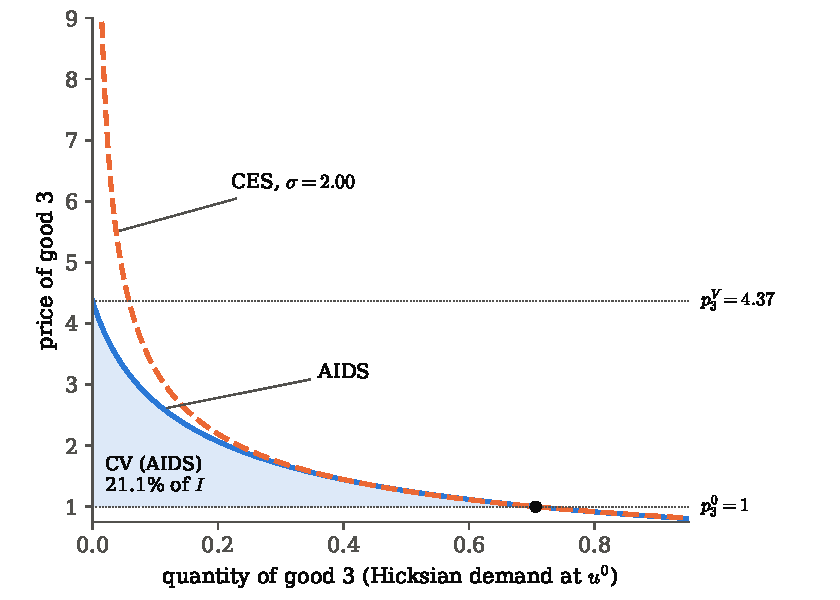
\includegraphics[width=0.78\textwidth]{figures/ch05/virtual_price.pdf}
\caption[Virtual price and the loss from removing a good]{Virtual price and the loss from removing a good.
The solid curve is the AIDS Hicksian demand for good 3 in the running example at the initial utility $u^0$,
with $p_1 = p_2 = 1$. It reaches zero at the virtual price $p_3^V = 4.37$. The shaded area is the compensating
variation of removing good 3, 21.1 percent of income. The dashed curve is the Hicksian demand of a CES system
calibrated to the same share ($0.26$) and own-price elasticity ($-1.738$) at the observed point. It approaches
the price axis only asymptotically, and the area to its left equals 35.2 percent of income. Computed with
\texttt{figures/ch05/src/virtual\_price.py}.}
\label{fig:05-virtual-price}
\end{figure}

\subsection{The extrapolation problem}\label{sec:05-welfare-extrapolation}

\begin{remark}[Virtual prices lie outside the data]\label{rem:05-extrapolation}
Every virtual-price calculation extrapolates. In the running example the virtual price is more than four times
the observed price. In Hausman's cereal data, prices vary by about 50 percent, while the estimated virtual
price is about twice the average price \citep[p.~228]{Hausman1997}. The answer is
then driven by the curvature of the chosen functional form beyond the support of the data. For AIDS the
relevant feature is the shape of shares in log prices, linear when $\beta_i = 0$ and quadratic otherwise.
\Cref{prop:05-variety}(c) shows how sensitive the
result is near unit elasticity: the log virtual price $\frac{1}{-\varepsilon_{ii} - 1}$ explodes as
$\varepsilon_{ii}$ approaches $-1$. \citet{Hausman1997} proposes a lower bound that needs only convexity of
demand: the tangent to the demand curve at the observed price meets the price axis below the true virtual price.
\Cref{ch:newgoods} develops this bound.
\end{remark}

\subsection{Recovering marginal costs from first-order conditions}\label{sec:05-welfare-supply}

Counterfactual prices require marginal costs, which are rarely observed. The standard approach inverts the
firms' pricing conditions, as in \cref{ch:theory} and \cref{ch:diffprod}. We state the conditions in
elasticity form, which is the natural form for product-space demand.

\casehead{Single-product pricing}
A firm that sets the price of product $i$ with constant marginal cost $c_i$ maximizes $(p_i - c_i)q_i(p)$. The
first-order condition is $q_i + (p_i - c_i)\frac{\partial q_i}{\partial p_i} = 0$. Dividing by $q_i$ and
multiplying by $\frac{1}{p_i}$ gives the Lerner condition
$\frac{p_i - c_i}{p_i} = -\frac{1}{\varepsilon_{ii}}$, and solving for the cost gives
\begin{equation}\label{eq:05-foc-single}
  c_i = p_i\Bigl(1 + \frac{1}{\varepsilon_{ii}}\Bigr).
\end{equation}
The condition is meaningful only when $\varepsilon_{ii} < -1$. A profit-maximizing firm never prices on the
inelastic part of its demand. The same condition holds for a product group whose price is set jointly by
perfectly colluding producers, the case used by \citet{ChaudhuriGoldbergJia2006}.

The elasticity in \eqref{eq:05-foc-single} must be \emph{unconditional}. It must include the reallocation of
expenditure across segments and between the category and other goods, computed by the chain rule of
\eqref{eq:05-uncond-elast}. A within-segment elasticity holds segment expenditure fixed. Suppose a segment's
own unconditional elasticity is below $-1$. Raising a brand's price then drains expenditure from the whole
segment, so the unconditional own elasticity is larger in magnitude than the conditional one. Markups computed from
conditional elasticities are then too high. \Cref{tab:05-hlz-own} shows this pattern for all fifteen beer
brands of \cref{sec:05-hlz}.

\casehead{Multiproduct pricing in elasticity form}
Firm $f$ owns the products in $\mathcal{J}_f$ and maximizes $\pi_f = \sum_{k\in\mathcal{J}_f}(p_k - c_k)q_k(p)$.
The first-order condition for $p_j$, $j\in\mathcal{J}_f$, is
\begin{equation*}
  q_j + \sum_{k\in\mathcal{J}_f}(p_k - c_k)\frac{\partial q_k}{\partial p_j} = 0.
\end{equation*}
Let $R_f = \sum_{k\in\mathcal{J}_f}p_kq_k$ be the firm's revenue, $r_k = \frac{p_kq_k}{R_f}$ the revenue share
of product $k$, and $\ell_k = \frac{p_k - c_k}{p_k}$ its Lerner index. Elsewhere the book writes $L$ for the
Lerner index. We write $\ell_k$ in this chapter, where $L$ denotes a likelihood. We multiply the condition by
$\frac{p_j}{R_f}$ and rewrite each term of the sum:
\begin{equation*}
  (p_k - c_k)\frac{\partial q_k}{\partial p_j}\frac{p_j}{R_f}
  = \frac{p_k - c_k}{p_k}\cdot\frac{p_kq_k}{R_f}\cdot\frac{\partial q_k}{\partial p_j}\frac{p_j}{q_k}
  = \ell_k\,r_k\,\varepsilon_{kj}.
\end{equation*}
The first-order conditions become
\begin{equation}\label{eq:05-foc-multi}
  r_j + \sum_{k\in\mathcal{J}_f}\ell_k\,r_k\,\varepsilon_{kj} = 0, \quad j\in\mathcal{J}_f,
  \qquad\text{or}\qquad r_f + E_f^\top m_f = 0.
\end{equation}
Here $r_f$ stacks the revenue shares and $m_f$ has elements $m_k = \ell_kr_k$. The matrix $E_f$ collects the
elasticities among the firm's products, with $(k,j)$ element $\varepsilon_{kj}$. Solving,
\begin{equation}\label{eq:05-markup-multi}
  m_f = -\bigl(E_f^\top\bigr)^{-1}r_f, \qquad \ell_k = \frac{m_k}{r_k}.
\end{equation}
This is the form in \citet[eqs.~7--9 and 14--15]{HausmanLeonardZona1994} and \citet[eqs.~12--15]{Hausman1997},
who write $s$ for the revenue shares and $w$ for $m_f$. The system is homogeneous of degree one in $r_f$, so
the shares can be normalized by any common revenue, such as total market revenue, without changing $\ell$.
Stacking all firms gives a block-diagonal elasticity matrix, one block per firm
\citep[eq.~14]{HausmanLeonardZona1994}.

The elasticity form is equivalent to the matrix markup formula of \cref{ch:diffprod}. Let $\Omega$ be the
ownership matrix and let $D$ have $(j,k)$ element $\frac{\partial q_k}{\partial p_j}$ (note the transposition
relative to the Jacobian of demand). Stacking the first-order conditions of all firms gives
\begin{equation*}
  q + (\Omega\odot D)(p - c) = 0, \qquad\text{so}\qquad p - c = -(\Omega\odot D)^{-1}q.
\end{equation*}
Dividing by market size turns quantities into market shares. Using $\frac{\partial q_k}{\partial p_j} =
\varepsilon_{kj}\frac{q_k}{p_j}$, row $j$ reads $q_j + \sum_k\Omega_{jk}\varepsilon_{kj}\frac{q_k}{p_j}(p_k - c_k) = 0$.
Multiplying by $\frac{p_j}{R_f}$ returns \eqref{eq:05-foc-multi}.

For a firm with two products, \eqref{eq:05-markup-multi} gives
\begin{equation}\label{eq:05-lerner-two}
  \ell_1 = \frac{-\varepsilon_{22} + \frac{r_2}{r_1}\varepsilon_{21}}{\varepsilon_{11}\varepsilon_{22} - \varepsilon_{12}\varepsilon_{21}}.
\end{equation}
With $\varepsilon_{21} = \varepsilon_{12} = 0$ this reduces to $-\frac{1}{\varepsilon_{11}}$. When the two
products are substitutes, the term $\frac{r_2}{r_1}\varepsilon_{21} > 0$ raises the markup on product 1. Part of
the demand lost by raising $p_1$ is recaptured by product 2. The size of the effect depends on the cross
elasticity of the sibling product with respect to $p_1$ and on its relative revenue.

\subsection{Partial identification of marginal cost}\label{sec:05-welfare-bounds}

The first-order condition \eqref{eq:05-foc-single} presumes a model of conduct. In many markets conduct is
unknown, and in regulated markets prices may not satisfy any unconstrained first-order condition.
\citet{ChaudhuriGoldbergJia2006} face both problems in the Indian antibiotics market (\cref{sec:05-cgj}).
Dozens of firms sell each molecule, and many prices are capped by regulation. Their solution is to bound
marginal cost instead of point-identifying it.

\begin{assumption}[Conduct between competition and joint monopoly]\label{ass:05-conduct-order}
For product group $i$ the following hold.
\begin{enumerate}[label=(\roman*)]
  \item Marginal cost $c_i$ is constant.
  \item Group demand $q_i(p_i,p_{-i})$ is differentiable, with $\frac{\partial q_i}{\partial p_i} < 0$.
  \item The group's joint profit $\Pi_i(p_i) = (p_i - c_i)q_i(p_i,p_{-i})$ is strictly quasi-concave in $p_i$,
  with maximizer $p_i^m$.
  \item The observed price satisfies $c_i \le p_i \le p_i^m$.
\end{enumerate}
\end{assumption}

Part (iv) is the substantive assumption. Prices are no lower than marginal cost, and no higher than the price a
joint monopolist of the group would choose given the other prices. Competition within the group and price
caps both move the price into this interval.

\begin{proposition}[Bounds on marginal cost]\label{prop:05-cost-bounds}
Under \cref{ass:05-conduct-order}, $c_i^L \le c_i \le c_i^U$, where
\begin{equation}\label{eq:05-cost-bounds}
  c_i^U = p_i, \qquad c_i^L = p_i\Bigl(1 + \frac{1}{\varepsilon_{ii}(p)}\Bigr),
\end{equation}
and $\varepsilon_{ii}(p)$ is the unconditional own-price elasticity at the observed prices. Equivalently,
$0 \le \ell_i \le -\frac{1}{\varepsilon_{ii}(p)}$.
\end{proposition}

\begin{proof}
The upper bound is the first inequality in part (iv). For the lower bound, a strictly quasi-concave function
increases up to its maximizer. Since $p_i \le p_i^m$, we have
$\Pi_i'(p_i) = q_i + (p_i - c_i)\frac{\partial q_i}{\partial p_i} \ge 0$. Rearranging,
$(p_i - c_i)\bigl(-\frac{\partial q_i}{\partial p_i}\bigr) \le q_i$. Dividing both sides by
$p_i\bigl(-\frac{\partial q_i}{\partial p_i}\bigr) > 0$ gives
\begin{equation*}
  \frac{p_i - c_i}{p_i} \le \frac{q_i}{p_i}\Bigl(-\frac{\partial q_i}{\partial p_i}\Bigr)^{-1} = -\frac{1}{\varepsilon_{ii}}.
\end{equation*}
Solving for $c_i$ gives $c_i \ge p_i\bigl(1 + \frac{1}{\varepsilon_{ii}}\bigr) = c_i^L$.
\end{proof}

These are equations (3.12) and (3.13) of \citet{ChaudhuriGoldbergJia2006}. Several remarks help in using them.
The lower bound is informative only when $\varepsilon_{ii} < -1$. If $-1 < \varepsilon_{ii} < 0$, then
$c_i^L < 0$ and the bound adds nothing to $c_i \ge 0$. The observed price then lies where demand is inelastic,
which no unconstrained joint monopolist would choose. That pattern is itself evidence of competition or
regulation. In the language of \cref{ch:conduct}, the bounds are the endpoints of the conduct-parameter model
$\frac{p_i - c_i}{p_i} = -\frac{\theta}{\varepsilon_{ii}}$ at $\theta = 0$ and $\theta = 1$. The bounds approach
avoids estimating $\theta$, which in a regulated market need not be a stable structural parameter. Bounds are
transparent, and they often suffice for a policy conclusion. In a counterfactual we simulate the outcome at
each bound. The two results bound the counterfactual outcome when that outcome is monotone in marginal cost,
which should be checked in each application.

\subsection{Counterfactual equilibrium after product withdrawal}\label{sec:05-counterfactual}

We now combine virtual prices, cost recovery and the multi-level demand system to simulate the withdrawal of
products. The setting is the two-level system of \cref{sec:05-separability}. An upper level allocates total
expenditure $X$ across segments $G$ with price indices $P_G$, and an AIDS allocates segment expenditure $X_Q$
within segment $Q$. A policy removes the products in $\mathcal{W}\subset Q$, and the products in
$\mathcal{R} = Q\setminus\mathcal{W}$ remain.

\casehead{The equilibrium system}
The unknowns are the virtual prices $p_i^V$ of the withdrawn products, the new prices $p_k'$ of the remaining
products, and the new segment expenditure and price index $X_Q'$ and $P_Q'$. They solve three blocks of
equations.
\begin{enumerate}[label=(S\arabic*)]
  \item Zero shares for withdrawn products. For each $i\in\mathcal{W}$,
  \begin{equation}\label{eq:05-cf-zero}
    0 = \alpha_i + \sum_{j\in\mathcal{W}}\gamma_{ij}\ln p_j^V + \sum_{k\in\mathcal{R}}\gamma_{ik}\ln p_k'
    + \beta_i\ln\frac{X_Q'}{P_Q'}.
  \end{equation}
  \item Pricing of remaining products. For single-product firms or colluding groups,
  \begin{equation}\label{eq:05-cf-price}
    p_k' = c_k\Bigl(1 + \frac{1}{\varepsilon_{kk}(p')}\Bigr)^{-1}, \quad k\in\mathcal{R},
  \end{equation}
  and for multiproduct firms the system \eqref{eq:05-foc-multi} evaluated at the new prices.
  \item Upper-level adjustment. The new index is $P_Q' = \mathbf{P}_Q(p^V_{\mathcal{W}},p'_{\mathcal{R}})$, and
  $X_Q'$ follows from the upper-level share equation of segment $Q$ evaluated at $P_Q'$ and the other segment
  indices.
\end{enumerate}
Equations~\eqref{eq:05-cf-zero} and \eqref{eq:05-cf-price} are equations (3.14) and (3.15) of \citet{ChaudhuriGoldbergJia2006},
written without their market-specific restrictions on the cross-price terms. The elasticities in (S2) are
unconditional and evaluated at the counterfactual prices, including the virtual prices.

One detail of (S2) deserves care. The demand that a remaining firm faces is AIDS demand evaluated at the
virtual prices, and by (S1) those prices move when $p_k'$ moves. For a single withdrawn product $i$, implicit
differentiation of $w_i = 0$ gives
$\frac{\partial\ln p_i^V}{\partial\ln p_j} = -\bigl(\frac{\partial w_i}{\partial\ln p_i}\bigr)^{-1}\frac{\partial w_i}{\partial\ln p_j}$.
The elasticity of demand for product $k$ with respect to $p_j$, once good $i$ has left, is therefore
\begin{equation}\label{eq:05-rationed-elast}
  \varepsilon_{kj}^{-i} = \varepsilon_{kj} - \varepsilon_{ki}\Bigl(\frac{\partial w_i}{\partial\ln p_i}\Bigr)^{-1}\frac{\partial w_i}{\partial\ln p_j},
\end{equation}
with all terms evaluated at $p_i^V$. This is the standard formula for demand under a ration of zero.

\casehead{Solving the system}
A simple algorithm iterates over the blocks. Start at the observed prices and expenditure. Given $p'_{\mathcal{R}}$
and $X_Q'$, solve (S1) for the virtual prices. Update $P_Q'$ and $X_Q'$ with (S3). Update $p'_{\mathcal{R}}$ with
(S2), using elasticities at the current prices. Repeat until the prices stop changing. Newton's method on the
stacked system converges faster when a good starting value is available. Existence and uniqueness are not
guaranteed, so we solve from several starting values and check the second-order conditions. We also verify
that the remaining shares stay positive and that the relevant own elasticities stay below $-1$.

\casehead{Welfare and its decomposition}
Let $E(u,P)$ be the upper-level expenditure function, with $P$ the vector of segment indices. Let $P^0$ be the
observed indices and $P'$ the counterfactual ones, with $P_Q'$ computed from the virtual and new prices. The
compensating variation is \citep[eq.~3.16]{ChaudhuriGoldbergJia2006}
\begin{equation}\label{eq:05-cv-cf}
  CV = E(u^0,P') - E(u^0,P^0).
\end{equation}
To see which mechanism drives it, define two intermediate price vectors. $P^1$ uses virtual prices computed with
$X_Q$ and all remaining prices fixed at their observed values. $P^2$ recomputes the virtual prices letting $X_Q$
respond to the new segment index, still holding the remaining prices fixed. Then
\begin{equation}\label{eq:05-cv-decomp}
  CV = \underbrace{E(u^0,P^1) - E(u^0,P^0)}_{\text{pure variety}}
  + \underbrace{E(u^0,P^2) - E(u^0,P^1)}_{\text{expenditure switching}}
  + \underbrace{E(u^0,P') - E(u^0,P^2)}_{\text{price adjustment}}.
\end{equation}
This is the general form of the decomposition used by \citet{ChaudhuriGoldbergJia2006}. The first term values
the lost products at fixed prices and fixed segment expenditure. The second term exists because the zero-share
condition (S1) is Marshallian. Whenever $\beta_i \neq 0$, the virtual prices depend on segment expenditure, so
they shift once $X_Q$ adjusts. The third term records the repricing of the remaining products. The first two
terms together describe a regime in which price regulation freezes the remaining prices at their old levels.
The decomposition is sequential, so its terms depend on the order in which the changes are introduced.

The welfare of a country adds producer surplus. With $\pi_k = (p_k - c_k)q_k$ computed at the counterfactual
and the observed prices, the change in national welfare is $-CV$ plus the change in the profits of domestic
firms. Profits of foreign firms are excluded from national welfare. They still measure the private gain that
motivates the policy. \Cref{sec:05-cgj-counterfactual} applies this accounting to patents in India.

\begin{example}[Withdrawal in the running example]\label{ex:05-withdrawal}
Treat the running example as a segment with fixed expenditure $X_Q = e$, sold by three single-product firms.
Equation~\eqref{eq:05-foc-single} recovers marginal costs $c = (0.273, 0.406, 0.425)$ from the observed prices and
elasticities. Suppose good 3 is withdrawn. Firms 1 and 2 reprice, facing the demand of consumers who can no
longer buy good 3, with its elasticities given by \eqref{eq:05-rationed-elast}. The new equilibrium has
$p_1' = 1.475$ and $p_2' = 1.365$, increases of 47.5 and 36.5 percent. The own elasticities fall in magnitude
from $-1.375$ and $-1.682$ to $-1.227$ and $-1.423$, because the closest outside option has gone. The total
compensating variation is 71.9 percent of segment expenditure. The pure variety effect, with other prices fixed,
is 21.1 percent (\cref{ex:05-virtual-running}). The price adjustment adds 50.8 percent. Firms 1 and 2 gain
$0.734$ in profit, while firm 3 loses $0.407$. These effects are large because fixing segment expenditure makes
the segment's aggregate demand unit elastic. An upper level with elastic segment demand would add the
expenditure-switching channel and dampen the price response. The computation is in \texttt{virtual\_price.py}.
\end{example}

\section{Case study: Hausman, Leonard and Zona (1994)}\label{sec:05-hlz}

\citet{HausmanLeonardZona1994} (HLZ) built the multi-level AIDS into a tool for antitrust analysis of
differentiated products. They estimated a three-level demand system for beer on store-level scanner data and
identified it with prices of the same brands in other cities. They then used the estimates to predict the price
effects of mergers and to test models of pricing. The paper is short and its data description is thin, but its
method shaped two decades of applied work. We treat it in depth.

\subsection{The economic question}\label{sec:05-hlz-question}

Antitrust questions about consumer goods turn on substitution among brands. Is a set of brands a market? Will
two brands owned by merging firms rise in price? Do observed markups match the predictions of a model of
competition? Each question needs own and cross elasticities for many brands. HLZ argue that the models then in
use restricted these elasticities too much. Representative-consumer models with symmetric preferences and
logit-type models share an \emph{independence of irrelevant alternatives} (IIA) property. Consumers of an
eliminated good spread over the remaining goods in proportion to their market shares. In terms
of elasticities, ``all cross price elasticities with respect to a given good are the same''
\citep[p.~160]{HausmanLeonardZona1994}. HLZ set out to estimate demand without such restrictions.

Store-level scanner data made this possible. Each transaction records units and price paid, by brand and by
stock-keeping unit, and weekly promotions generate large price variation. Two econometric problems remain. The
first is dimensionality. It is ``difficult to conceive of estimating a demand equation with say 135 brands of
cereal or say 40 brands of beer'' (p.~160). The second is identification: at the brand level, cost shifters that
vary across brands and weeks are hard to find. HLZ answer the first problem with multi-stage budgeting and the
second with prices in other cities.

A third theme runs through the applications. Firms in these industries sell many brands. HLZ list Miller High
Life, Miller Lite, Miller Genuine Draft, Milwaukee's Best and Meisterbrau as Miller brands, and note that
Kellogg's produces over 30 cereals (p.~161). A multiproduct firm that raises one brand's price recaptures some
of the lost sales on its other brands. HLZ show how this \emph{cannibalization} changes merger predictions and
tests of conduct.

\subsection{Setting and data}\label{sec:05-hlz-data}

Marketing analysts divide the U.S. beer market into segments: premium, light (low-calorie), imported and
popular-price beer (p.~162). In estimation HLZ use three segments. The premium segment includes imported
beers, which they found belong with premium brands (p.~164). Each segment contains five brands, for fifteen
brands in total (\cref{fig:05-hlz-tree}). The brands include national brands such as Budweiser, Miller and
Coors, Canadian imports such as Molson and Labatts, and regional brands such as Genesee.

\begin{figure}[htbp]
\centering
\begin{tikzpicture}[
  every node/.style={font=\small},
  seg/.style={draw, rounded corners=2pt, minimum width=2.6cm, inner sep=3pt, fill=gray!8},
  brands/.style={align=center, font=\footnotesize, text width=3.3cm}]
  \node[seg, minimum width=3.4cm] (beer) at (0,0) {Beer (top level)};
  \node[seg] (prem) at (-4.6,-1.6) {Premium};
  \node[seg] (pop)  at (0,-1.6)    {Popular price};
  \node[seg] (lig)  at (4.6,-1.6)  {Light};
  \foreach \s in {prem,pop,lig} \draw[-{Latex[length=2mm]}] (beer.south) -- (\s.north);
  \node[brands, anchor=north] (b1) at (-4.6,-2.2) {Budweiser\\ Molson\\ Labatts\\ Miller\\ Coors};
  \node[brands, anchor=north] (b2) at (0,-2.2) {Old Milwaukee\\ Genesee\\ Milwaukee's Best\\ Busch\\ Piels Lager};
  \node[brands, anchor=north] (b3) at (4.6,-2.2) {Genesee Light\\ Coors Light\\ Old Milwaukee Light\\ Lite\\ Molson Light};
  \foreach \s/\b in {prem/b1,pop/b2,lig/b3} \draw[-{Latex[length=2mm]}] (\s.south) -- (\b.north);
  \node[anchor=west, font=\footnotesize\itshape] at (6.6,0) {top};
  \node[anchor=west, font=\footnotesize\itshape] at (6.6,-1.6) {middle};
  \node[anchor=west, font=\footnotesize\itshape] at (6.6,-3.2) {bottom};
\end{tikzpicture}
\caption[The three-level budgeting tree of Hausman, Leonard and Zona]{The three-level budgeting tree of
\citet{HausmanLeonardZona1994}. The top level determines beer consumption relative to other goods, the middle
level allocates beer expenditure across three segments, and the bottom level allocates each segment's
expenditure across five brands. Imported beers are included in the premium segment. Brand lists from HLZ,
Tables 2 to 5.}
\label{fig:05-hlz-tree}
\end{figure}

The data are cash-register records from individual stores, aggregated to the metropolitan area (SMSA) level.
For each brand they give sales and price per unit, after aggregating over container sizes (p.~160). Most price
variation comes from supermarket chains running low-price promotions on a brand in a given week (p.~167).
In most cases manufacturers sell at wholesale nationally, with a uniform wholesale price (p.~161), which
motivates the
identification strategy below. The paper reports little else about the sample. Two graphs show weekly sales of
Budweiser and Genesee in Buffalo in February and March 1988 and in March to June 1990. The middle-level
regressions of Table 1 use 101 observations. HLZ do not report the list of cities, the sample period or the
number of stores. The top level uses national monthly data from the Bureau of Labor Statistics covering
sixteen years (p.~164). The share equations also include a time trend and the log number of stores.

\subsection{The three-level demand model}\label{sec:05-hlz-model}

HLZ apply the multi-stage budgeting framework of \cref{sec:05-separability} with three levels. We write their
equations in this chapter's notation. Cities are indexed by $n = 1,\dots,N$ (in this section $N$ counts cities)
and weeks by $t$. Segments are $G$ and $H$, and brands are $i$ and $j$.

\casehead{Bottom level: brands within a segment}
For brand $i$ in segment $G$,
\begin{equation}\label{eq:05-hlz-bottom}
  w_{int} = \alpha_{in} + \beta_i\ln\frac{X_{Gnt}}{P_{Gnt}} + \sum_{j\in G}\gamma_{ij}\ln p_{jnt} + \xi_{int}.
\end{equation}
This is equation (1) of \citet{HausmanLeonardZona1994}. Here $w_{int}$ is the revenue share of brand $i$ in segment expenditure
$X_{Gnt}$, $P_{Gnt}$ is a segment price index and $p_{jnt}$ is the price of brand $j$. The intercept
$\alpha_{in}$ is a brand-city effect. This is an AIDS for the segment, with symmetry
$\gamma_{ij} = \gamma_{ji}$ imposed in estimation. The $\gamma_{ij}$ are free within the segment, so no IIA-type
restriction constrains the cross elasticities among the brands that compete most closely. A test of
$\beta_i = 0$ is a test of segment homotheticity. HLZ stress that the expenditure variable must be segment
expenditure (p.~163), in the words that \citet{Hausman1997} repeats and that we quoted in
\cref{sec:05-second-stage}.

\casehead{Middle level: segments}
Given the bottom-level estimates, HLZ construct a price index for each segment. They use either the exact index
implied by the bottom-level expenditure function or a weighted-average index of the Laspeyres type, and report
that the choice matters little (p.~164). The segment demands are log-log:
\begin{equation}\label{eq:05-hlz-middle}
  \ln q_{Gnt} = \alpha_{Gn} + \beta_G\ln X_{Bnt} + \sum_{H}\vartheta_{GH}\ln P_{Hnt} + \xi_{Gnt},
\end{equation}
where $q_{Gnt}$ is the quantity of segment $G$ and $X_{Bnt}$ is total beer expenditure (HLZ eq.~2, where
the price coefficients are written $\delta_k$). Because beer expenditure is held fixed, $\beta_G$ and
$\vartheta_{GH}$ are conditional elasticities. Slutsky restrictions are not imposed at this level (fn.~3).
Exact two-stage budgeting under Gorman's results, discussed in \citet{BlackorbyPrimontRussell1978}, requires
additive separability at the level above. HLZ note
that AIDS is a generalized Gorman polar form, so Gorman's theorem applies, and that a less restrictive middle
level, not consistent with exact two-stage budgeting, gives similar results (fn.~2).

\casehead{Top level: beer}
Overall beer consumption $Q_{Bt}$ is
\begin{equation}\label{eq:05-hlz-top}
  \ln Q_{Bt} = \varphi_0 + \varphi_1\ln y_t + \varphi_2\ln P_{Bt} + Z_t^\top\psi + \xi_{Bt}.
\end{equation}
This is HLZ's equation (3). Here $y_t$ is deflated disposable income and $P_{Bt}$ is the deflated beer price index. The vector
$Z_t$ holds demographics, monthly seasonal factors and the minimum legal age for buying beer. The coefficient
$\varphi_2$ is the overall price elasticity of beer. HLZ estimate it by instrumental variables on the national
monthly data, with cost shifters for ingredients, packaging and labor as instruments.

\casehead{From three levels to unconditional elasticities}
Estimation runs bottom-up, and the elasticities that matter for competition combine all three levels. The
two-level chain rule of \eqref{eq:05-uncond-elast} extends directly. Take brand $i$ in segment $G$ and brand $j$
in segment $H$, and drop the city and week subscripts. Let $\varepsilon_{ij}\big|_{X_G}$ be the
within-segment elasticity at fixed segment expenditure and $\eta_{i\mid G} = 1 + \frac{\beta_i}{w_i}$ the
elasticity of brand $i$ with respect to segment expenditure. Then
\begin{equation*}
  \varepsilon_{ij} = \indic(G = H)\,\varepsilon_{ij}\big|_{X_G} + \eta_{i\mid G}\,\frac{\partial\ln X_G}{\partial\ln p_j}.
\end{equation*}
Segment expenditure is $X_G = P_Gq_G$, so $\ln X_G = \ln P_G + \ln q_G$. The index $P_G$ responds to $p_j$ only
if $H = G$. The quantity $q_G$ responds through the price index $P_H$ and through beer expenditure:
\begin{equation*}
  \frac{\partial\ln q_G}{\partial\ln p_j} = \Bigl[\vartheta_{GH} + \beta_G\frac{\partial\ln X_B}{\partial\ln P_H}\Bigr]\frac{\partial\ln P_H}{\partial\ln p_j}.
\end{equation*}
Beer expenditure is $X_B = P_BQ_B$, and with income fixed the top level gives
$\frac{\partial\ln X_B}{\partial\ln P_B} = 1 + \varphi_2$. If the beer index has segment weights $w_H$ (the shares
of the segments in beer expenditure), then $\frac{\partial\ln P_B}{\partial\ln P_H} = w_H$. Collecting terms,
\begin{equation}\label{eq:05-hlz-uncond}
  \varepsilon_{ij} = \indic(G = H)\,\varepsilon_{ij}\big|_{X_G}
  + \eta_{i\mid G}\Bigl[\indic(G = H) + \vartheta_{GH} + \beta_G(1 + \varphi_2)w_H\Bigr]\frac{\partial\ln P_H}{\partial\ln p_j}.
\end{equation}
For a Stone or Laspeyres segment index, $\frac{\partial\ln P_H}{\partial\ln p_j}$ is the weight of brand $j$ in
the index. For the exact translog index it equals $w_j - \beta_j\ln\frac{X_H}{P_H}$ (\cref{sec:05-aids}).

Equation~\eqref{eq:05-hlz-uncond} has two consequences. For the own elasticity ($j = i$), the bracket equals
$1 + \vartheta_{GG} + \beta_G(1 + \varphi_2)w_G$. It is negative whenever the segment's own conditional
elasticity is well below $-1$, as it is in the beer data. The unconditional own elasticity is then larger in
magnitude than the conditional one. For brands in different segments, $\varepsilon_{ij}$ depends on brand $j$
only through its weight in index $H$, and on brand $i$ only through $\eta_{i\mid G}$. All brand-pair specific
substitution across segments is ruled out. This is the price of the dimension reduction.

The restriction has a compensated counterpart. By the theorem of \citet{GoldmanUzawa1964}
(\cref{prop:05-goldman-uzawa}), weak separability implies $S_{ij} = \mu_{GH}\frac{\partial q_i}{\partial I}\frac{\partial q_j}{\partial I}$
for $i\in G$, $j\in H$, $G\neq H$. To convert to elasticities, we use
$\frac{\partial q_i}{\partial I} = \frac{\partial q_i}{\partial X_G}\frac{\partial X_G}{\partial I}
= \eta_{i\mid G}\frac{q_i}{X_G}\frac{\partial X_G}{\partial I}$ and the same expression for good $j$ in segment $H$.
Then
\begin{equation*}
  \varepsilon^h_{ij} = \frac{p_j}{q_i}S_{ij}
  = \mu_{GH}\,\eta_{i\mid G}\,\eta_{j\mid H}\,\frac{\partial X_G}{\partial I}\frac{\partial X_H}{\partial I}\,
    \frac{p_jq_j}{X_GX_H},
\end{equation*}
which gives
\begin{equation*}
  \varepsilon^h_{ij} = \lambda_{GH}\,w_{j\mid H}\,\eta_{i\mid G}\,\eta_{j\mid H},
  \qquad \lambda_{GH} = \frac{\mu_{GH}}{X_G}\frac{\partial X_G}{\partial I}\frac{\partial X_H}{\partial I},
\end{equation*}
where $w_{j\mid H}$ is the share of brand $j$ in segment $H$ and $\lambda_{GH}$ depends only on the pair of
segments. HLZ state the restriction as $\varepsilon^h_{ij} = \lambda_{GH}\eta_{i\mid G}\eta_{j\mid H}$
\citep[eq.~5]{HausmanLeonardZona1994}. The exact conversion adds the within-segment share of brand $j$. Either
way, a segment-pair constant and brand-level expenditure elasticities determine all compensated substitution
across segments.

The dimension reduction is large. A complete AIDS for fifteen brands has $\frac{15 \times 14}{2} = 105$ free
price coefficients after symmetry and homogeneity. Three five-brand segments have $3 \times 10 = 30$, the middle
level adds nine segment price elasticities, and the top level adds one.

\subsection{Identification with prices in other cities}\label{sec:05-hlz-identification}

Prices in \eqref{eq:05-hlz-bottom} are endogenous if retailers and manufacturers set them knowing local demand
conditions. Cost shifters that vary by brand and week are rarely available. An ``insufficient number of input
prices may exist or they may not be reported with high enough frequency'' (p.~164). HLZ exploit the panel
structure of the data instead. They model the price of brand $j$ in city $n$ and week $t$ as
\begin{equation}\label{eq:05-hlz-price}
  \ln p_{jnt} = \rho_j\ln c_{jt} + \mu_{jn} + \zeta_{jnt}.
\end{equation}
This is HLZ's equation (4), with our $\rho_j$, $\mu_{jn}$ and $\zeta_{jnt}$ in place of their $\delta_j$,
$\alpha_{jn}$ and $w_{jnt}$. Here $c_{jt}$ is the cost of brand $j$, assumed to have no
city-specific time variation, consistent with national shipments and advertising. The term $\mu_{jn}$ is a
city-brand differential reflecting transport costs or local wages. The shock $\zeta_{jnt}$ has mean zero and
captures local promotions.

\begin{assumption}[Prices in other cities as instruments]\label{ass:05-hausman-iv}
In \eqref{eq:05-hlz-price} the following hold.
\begin{enumerate}[label=(\roman*)]
  \item The cost component $c_{jt}$ is common to all cities.
  \item The city-brand effects $\mu_{jn}$ are constant over time.
  \item The local shocks $\zeta_{jnt}$ are independent across cities. They may be correlated across brands
  within a city \citep[fn.~19]{Hausman1997}.
  \item The demand errors $\xi_{int}$ are uncorrelated with the cost component and with the local price shocks
  of other cities.
\end{enumerate}
\end{assumption}

Let a tilde denote the deviation from the city-brand mean, the within transformation that removes $\mu_{jn}$
and the fixed effects in \eqref{eq:05-hlz-bottom}. Under \cref{ass:05-hausman-iv} the prices of every brand of
the segment in any other city $n'\neq n$ satisfy the moment conditions
\begin{equation}\label{eq:05-hausman-iv}
  \E\bigl[\tilde\xi_{int}\,\widetilde{\ln p}_{jn't}\bigr] = 0, \qquad j\in G,\ n'\neq n.
\end{equation}
Instruments of this kind are now called \emph{Hausman instruments}. Relevance and exclusion follow from
\eqref{eq:05-hlz-price}. The price in city $n'$ shares the cost component with the price in city $n$, while the
local shocks are independent, so
\begin{equation*}
  \Cov\bigl(\widetilde{\ln p}_{jn't},\widetilde{\ln p}_{jnt}\bigr) = \rho_j^2\Var\bigl(\widetilde{\ln c}_{jt}\bigr) > 0
\end{equation*}
whenever national costs vary over time. The covariance with the demand error is
\begin{equation*}
  \Cov\bigl(\widetilde{\ln p}_{jn't},\tilde\xi_{int}\bigr)
  = \rho_j\Cov\bigl(\widetilde{\ln c}_{jt},\tilde\xi_{int}\bigr) + \Cov\bigl(\tilde\zeta_{jn't},\tilde\xi_{int}\bigr),
\end{equation*}
and both terms are zero by part (iv). In words, ``prices in one city (after elimination of city and brand specific effects)
are driven by underlying costs'' (p.~165).

The first stage regresses $\ln p_{jnt}$ on the brand-city effects, the exogenous regressors and the prices of the
segment's brands in other cities, either city by city or averaged. With more than two cities the model is
overidentified, and HLZ point to the tests of \citet{HausmanTaylor1981} for checking the instrument assumptions
(fn.~4). The logic is that of \citet{HausmanTaylor1981}: after unit effects are removed, variation shared with
other units serves as an instrument. The share equations are estimated as a system, as the residual covariance
matrices reported with Tables 2 to 4 suggest, and symmetry is imposed across equations.

HLZ also offer a second interpretation. Suppose supermarkets set weekly prices under constant short-run marginal
cost and do not adjust them to clear the market. Prices are then predetermined with respect to the demand errors,
and ordinary least squares is consistent. Segment expenditure $X_{Gnt}$ may still need instruments, since it
responds to the same demand shocks. The choice between the two views can be tested with the specification test
of \citet{Hausman1978}. That test compares the IV and OLS estimates through
\begin{equation*}
  \mathcal{H} = (\hat b_{IV} - \hat b_{OLS})^\top\bigl[\widehat{\Var}(\hat b_{IV}) - \widehat{\Var}(\hat b_{OLS})\bigr]^{-1}(\hat b_{IV} - \hat b_{OLS}),
\end{equation*}
which is asymptotically chi-squared under exogeneity, with degrees of freedom equal to the number of
coefficients tested. HLZ describe the test but do not report its outcome for beer.

Later work adopted these instruments widely. \citet{Nevo2001} uses regional quarterly average prices of the same
brand, excluding the city being instrumented, in his study of breakfast cereals. \Cref{ch:logit} and
\cref{ch:blp} return to them.

\subsection{Validity: Bresnahan's critique}\label{sec:05-bresnahan-critique}

The identifying assumption rules out demand shocks that are common across cities and reflected in prices.
\citet{Bresnahan1997} made this objection in his comment on \citet{Hausman1997}, which uses the same strategy for
cereals. For the assumption to hold, ``there can be no successful nationwide advertising campaigns which shift
the demand for individual brands or products'' \citep[p.~241]{Bresnahan1997}. There can be no national fads and
no slow national acceptance of new brands. Adding advertising to the demand equation does not settle the issue,
because the econometrician does not observe which campaigns succeed (fn.~6). The fallback that prices are
predetermined requires such shocks to be unforeseen when prices are set, which Bresnahan finds unlikely for
national campaigns. If national shocks exist and supply slopes up, prices in other cities move with the demand
error. Supply can slope up in the one-week run because inventories cannot adjust or because of market power
(fn.~7).

\casehead{The bias with one product}
We derive the bias in the simplest version of Bresnahan's model: one product, linear demand, single-product
Bertrand pricing and constant marginal cost. In city $n$ and week $t$,
\begin{equation*}
  q_{nt} = d + a\,p_{nt} + \xi_{nt}, \quad a < 0, \qquad\qquad p_{nt} = c_{nt} + \frac{q_{nt}}{-a}.
\end{equation*}
The pricing equation is the first-order condition $q + (p - c)a = 0$. Substituting demand into it gives
$p = c - \frac{d}{a} - p - \frac{\xi}{a}$, so
\begin{equation*}
  p_{nt} = \frac{1}{2}c_{nt} - \frac{d + \xi_{nt}}{2a}.
\end{equation*}
Let the demand error have a national and a local part, $\xi_{nt} = \chi_t + e_{nt}$, and let cost have the same
structure, $c_{nt} = \bar c_t + v_{nt}$. The national components have variances $\sigma_\chi^2$ and $\sigma_c^2$.
All components are mutually independent, and the local ones are independent across cities. The instrument for
$p_{nt}$ is $p_{n't}$ with $n'\neq n$. Only the national components survive in the covariances:
\begin{equation*}
  \Cov(p_{n't},\xi_{nt}) = -\frac{\sigma_\chi^2}{2a}, \qquad
  \Cov(p_{n't},p_{nt}) = \frac{\sigma_c^2}{4} + \frac{\sigma_\chi^2}{4a^2}.
\end{equation*}
The IV estimator therefore converges to
\begin{equation}\label{eq:05-iv-bias-scalar}
  \plim\hat a = a + \frac{\Cov(p_{n't},\xi_{nt})}{\Cov(p_{n't},p_{nt})}
  = a - \frac{2a\,\sigma_\chi^2}{a^2\sigma_c^2 + \sigma_\chi^2} = a(1 - 2\lambda),
  \qquad \lambda = \frac{\sigma_\chi^2}{a^2\sigma_c^2 + \sigma_\chi^2}.
\end{equation}
The weight $\lambda\in[0,1]$ is the share of national demand shocks in the price variation common to all
cities. Without national demand shocks ($\lambda = 0$) the estimator is consistent. Otherwise the estimate lies
between $a$ and $-a$, biased toward zero, so demand looks too steep. When $\lambda > \frac{1}{2}$ the estimated
slope even has the wrong sign. At $\lambda = 1$ the estimator recovers $-a$, the slope of the supply relation
$q = -a(p - c)$. In Bresnahan's words, the estimator then behaves ``like doing ordinary least squares on a supply
and demand system'' (p.~242).

\casehead{The bias with many products}
The same logic extends to $J$ products, and the exact bias has a compact form. Let demand be
$q_{nt} = d + A\,p_{nt} + \xi_{nt}$, with $A = [a_{jk}]$ and $a_{jk} = \frac{\partial q_j}{\partial p_k}$. Single-product
Bertrand pricing gives $p_{jnt} = c_{jnt} + \frac{q_{jnt}}{-a_{jj}}$, or $p = c + \Theta^{-1}q$ with
$\Theta = \diag(-a_{11},\dots,-a_{JJ})$. Multiplying by $\Theta$ and substituting demand,
\begin{equation*}
  \Theta p_{nt} = \Theta c_{nt} + d + Ap_{nt} + \xi_{nt}, \qquad\text{so}\qquad p_{nt} = (\Theta - A)^{-1}\bigl(d + \Theta c_{nt} + \xi_{nt}\bigr).
\end{equation*}
This is the price system in the appendix of \citet{Bresnahan1997}. Let the national demand and cost components
have covariance matrices $\Sigma_\chi$ and $\Sigma_c$, and write $M = (\Theta - A)^{-1}$. Equation $j$ is estimated
by IV with the vector of other-city prices $p_{n't}$ as instruments. Its coefficient vector, the transpose of
row $j$ of $A$, converges to $A_{j\cdot}^\top + [\E(\tilde p_{n't}\tilde p_{nt}^\top)]^{-1}\E(\tilde p_{n't}\xi_{jnt})$.
The two moments are
\begin{equation*}
  \E(\tilde p_{n't}\tilde p_{nt}^\top) = M\bigl(\Theta\Sigma_c\Theta + \Sigma_\chi\bigr)M^\top, \qquad
  \E(\tilde p_{n't}\xi_{jnt}) = M\Sigma_\chi\mathbf{e}_j,
\end{equation*}
where $\mathbf{e}_j$ is the $j$th unit vector. The bias of equation $j$ is therefore
$(\Theta - A)^\top(\Theta\Sigma_c\Theta + \Sigma_\chi)^{-1}\Sigma_\chi\mathbf{e}_j$. Stacking the equations and using the symmetry of
the covariance matrices gives the following result.

\begin{proposition}[Bias of other-city price instruments]\label{prop:05-iv-bias}
In the linear model above, IV estimation with other-city prices satisfies
\begin{equation}\label{eq:05-iv-bias}
  \plim\hat A = (I - \Lambda)A + \Lambda\Theta, \qquad \Lambda = \Sigma_\chi\bigl(\Theta\Sigma_c\Theta + \Sigma_\chi\bigr)^{-1}.
\end{equation}
The estimate is a matrix-weighted average of the demand slopes $A$ and the supply slopes $\Theta$. With
$\Sigma_\chi = 0$ it is consistent, and with $\Sigma_c = 0$ it recovers $\Theta$, which has own slopes $-a_{jj}$ and
zero cross slopes.
\end{proposition}

When the national demand and cost shocks are uncorrelated across products, $\Lambda = \diag(\lambda_1,\dots,\lambda_J)$ with
$\lambda_j = \frac{\sigma_{\chi j}^2}{a_{jj}^2\sigma_{cj}^2 + \sigma_{\chi j}^2}$. Then
$\plim\hat a_{jj} = (1 - 2\lambda_j)a_{jj}$ and $\plim\hat a_{jk} = (1 - \lambda_j)a_{jk}$. Own slopes are biased
toward zero as in the one-product case, and cross slopes are attenuated toward zero. Correlated national shocks
change the cross terms. The bias of $a_{12}$ is $-\Lambda_{11}a_{12} - 2\Lambda_{12}a_{22}$, and the second term is
positive when $\Lambda_{12} > 0$. Cross slopes can then be inflated. \texttt{bresnahan\_bias\_check.py} confirms
\eqref{eq:05-iv-bias} by simulation. For example, with $A = \bigl[\begin{smallmatrix}-2 & 0.5\\ 0.5 & -1.5\end{smallmatrix}\bigr]$,
$\Sigma_c = 0.3I$ and $\Sigma_\chi = 0.4I$, the probability limit is
$\bigl[\begin{smallmatrix}-1.00 & 0.375\\ 0.314 & -0.384\end{smallmatrix}\bigr]$. If the national shocks have
correlation $0.8$ across the two products, it becomes
$\bigl[\begin{smallmatrix}-1.31 & 1.11\\ 0.87 & -0.57\end{smallmatrix}\bigr]$.

\casehead{Bresnahan's printed result}
Bresnahan states that the sign and magnitude of the bias are governed by $\Sigma_\chi[\diag(-\gamma) - \gamma]^{-1}$,
in his notation $\gamma_{jk} = a_{jk}$. This matrix is the covariance between other-city prices and demand
errors, $M\Sigma_\chi$ up to transposition. For two products whose national shocks have correlation $\varrho$, his
appendix (pp.~246--247) reports the elements
\begin{equation*}
  \frac{\sigma}{4\gamma_{11}\gamma_{22} - \gamma_{12}\gamma_{21}}
  \begin{bmatrix} -2\gamma_{22} + \varrho\gamma_{21} & \gamma_{12} - 2\varrho\gamma_{11}\\
  -2\varrho\gamma_{22} + \gamma_{21} & \varrho\gamma_{12} - 2\gamma_{11}\end{bmatrix}.
\end{equation*}
He concludes that the on-diagonal bias has the sign of
$-2\gamma_{22} + \varrho\gamma_{12}$ and the off-diagonal bias the sign of $\gamma_{12} - 2\varrho\gamma_{11}$. At
$\varrho = 0$ these are positive: own coefficients are biased toward zero and cross coefficients away from zero.
The printed algebra has typographical slips. The intermediate inverse has the wrong signs off the diagonal,
although the final matrix is correct, and the text writes $\varrho\gamma_{12}$ where the matrix has
$\varrho\gamma_{21}$, which coincide under symmetry. The reading of covariance signs as bias signs is exact with
one price. With several endogenous prices the bias also involves the inverse of the first-stage covariance
matrix, as \eqref{eq:05-iv-bias} shows. With $\varrho = 0$ the cross coefficients are attenuated, while
sufficiently correlated national shocks inflate them. Bresnahan's footnote 9 already hedges the cross-price
claim, saying that it ``depends on the covariances of the shocks to demand across products.'' Correlated
national shocks can also bias an own slope away from zero. The bias of $a_{jj}$ is the diagonal element
$2\Lambda_{jj}|a_{jj}| - \sum_{k\neq j}\Lambda_{jk}a_{kj}$ of $\Lambda(\Theta - A)$, and the second term can dominate.
With the matrix $A$ above, $\Sigma_c = \diag(5, 0.01)$ and
$\Sigma_\chi = 0.4\bigl[\begin{smallmatrix}1 & 0.95\\ 0.95 & 1\end{smallmatrix}\bigr]$ give
$\plim\hat a_{11} = -2.44$, farther from zero than the true $-2$. The own-price bias toward zero holds when
$2\Lambda_{jj}|a_{jj}| > \sum_{k\neq j}\Lambda_{jk}a_{kj}$, for example when national demand and cost shocks are
uncorrelated across products.

\casehead{What the critique implies}
National demand shocks typically make estimated own elasticities too small in magnitude. Markups recovered from
\eqref{eq:05-foc-multi} are then too high, simulated merger price increases too large, and the value of new goods
too large. Bresnahan's own concern was the last of these. \citet[fn.~25]{Hausman1997} anticipates the objection
by citing the beer estimates of HLZ, whose own-price elasticities lie ``in the range of about $-4.0$ to $-6.2$''.
He concludes that the method does not mechanically produce small elasticities. The reply is incomplete. A bias
toward zero is compatible with large estimates if the true elasticities are larger still. The assumption can be
probed in the data. Overidentification tests across cities are one check. A more direct symptom of national
shocks is correlation between the demand residuals of the same brand in different cities in the same week.
Instruments based on observed local cost variation offer a comparison, as in \citet{Nevo2001}. Bresnahan
himself points to other approaches to estimating substitution, including the then recent method of
\citet{Berry1994} (fn.~10). The critique
applies to every use of Hausman instruments, including random-coefficient models (\cref{ch:blp}).

\subsection{Results}\label{sec:05-hlz-results}

\casehead{Top and middle levels}
The overall price elasticity of beer is $-1.36$, with standard error 0.21 (p.~164). \Cref{tab:05-hlz-table1}
reproduces the segment equations. Each column is a segment demand equation, and because the equations are
log-log, the coefficients are conditional elasticities. Expenditure elasticities are close to one. The own
price elasticities are about $-2.7$ for premium and popular-price beer and $-2.4$ for light beer. These are large
for segment-level elasticities. They imply that a hypothetical attempt to raise all premium prices would not pay
if light and popular prices stayed put (p.~166).

\begin{table}[htbp]
\centering
\caption{Segment demand equations for beer}\label{tab:05-hlz-table1}
\begin{threeparttable}
\begin{tabular}{@{}lccc@{}}
\toprule
 & Premium & Popular & Light \\
\midrule
Constant & $0.501$ & $-4.021$ & $-1.183$ \\
 & $(0.283)$ & $(0.560)$ & $(0.377)$ \\
$\ln$ beer expenditure & $0.978$ & $0.943$ & $1.067$ \\
 & $(0.011)$ & $(0.022)$ & $(0.015)$ \\
$\ln P_{\text{premium}}$ & $-2.671$ & $2.704$ & $0.424$ \\
 & $(0.123)$ & $(0.244)$ & $(0.166)$ \\
$\ln P_{\text{popular}}$ & $0.510$ & $-2.707$ & $0.747$ \\
 & $(0.097)$ & $(0.193)$ & $(0.127)$ \\
$\ln P_{\text{light}}$ & $0.701$ & $0.518$ & $-2.424$ \\
 & $(0.070)$ & $(0.140)$ & $(0.092)$ \\
Time & $-0.001$ & $-0.000$ & $0.002$ \\
 & $(0.000)$ & $(0.001)$ & $(0.000)$ \\
$\ln$ number of stores & $-0.035$ & $0.253$ & $-0.176$ \\
 & $(0.016)$ & $(0.034)$ & $(0.023)$ \\
\midrule
Observations & \multicolumn{3}{c}{101} \\
\bottomrule
\end{tabular}
\begin{tablenotes}[flushleft]\footnotesize
\item Notes: Dependent variable is the log quantity of the segment, \eqref{eq:05-hlz-middle}. Each column is one
equation. Coefficients on log prices are elasticities conditional on beer expenditure. Standard errors in
parentheses. Source: \citet[Table 1]{HausmanLeonardZona1994}.
\end{tablenotes}
\end{threeparttable}
\end{table}

The cross elasticities are large and positive. A 10 percent rise in the premium price index raises light-beer
demand by about 4.2 percent, and the popular-price equation has a coefficient of 2.70 on the premium index. HLZ
draw an antitrust conclusion. Claims that segments such as light and popular beer form separate markets are
contradicted by the data, because enough marginal consumers switch segments in response to price (p.~166).

\casehead{Bottom level}
\Cref{tab:05-hlz-table2} reproduces the premium-segment share equations. The AIDS coefficients are not
elasticities, so HLZ report the implied conditional own-price elasticities in the last row. Premium brands have
conditional own elasticities between $-3.5$ and $-5.0$. The conditional cross elasticities of Budweiser lie
between 0.4 and 1.0, and Coors has a conditional cross elasticity of 1.0 with respect to Labatts (p.~166). The
coefficients on $\ln\frac{X}{P}$ are small. HLZ describe income effects at the bottom level as very small
(p.~169).

\begin{table}[htbp]
\centering
\caption{Brand share equations, premium segment}\label{tab:05-hlz-table2}
\begin{threeparttable}
\begin{tabular}{@{}lccccc@{}}
\toprule
 & Budweiser & Molson & Labatts & Miller & Coors \\
\midrule
Constant & $0.393$ & $0.377$ & $0.230$ & $-0.104$ & \\
 & $(0.062)$ & $(0.078)$ & $(0.056)$ & $(0.031)$ & \\
Time & $0.001$ & $-0.000$ & $0.001$ & $0.000$ & \\
 & $(0.000)$ & $(0.000)$ & $(0.000)$ & $(0.000)$ & \\
$\ln\frac{X}{P}$ & $-0.004$ & $-0.011$ & $-0.006$ & $0.017$ & \\
 & $(0.006)$ & $(0.007)$ & $(0.005)$ & $(0.003)$ & \\
$\ln p_{\text{Budweiser}}$ & $-0.936$ & $0.372$ & $0.243$ & $0.150$ & \\
 & $(0.041)$ & $(0.231)$ & $(0.034)$ & $(0.018)$ & \\
$\ln p_{\text{Molson}}$ & $0.372$ & $-0.804$ & $0.183$ & $0.130$ & \\
 & $(0.231)$ & $(0.031)$ & $(0.022)$ & $(0.012)$ & \\
$\ln p_{\text{Labatts}}$ & $0.243$ & $0.183$ & $-0.588$ & $0.028$ & \\
 & $(0.034)$ & $(0.022)$ & $(0.044)$ & $(0.019)$ & \\
$\ln p_{\text{Miller}}$ & $0.150$ & $0.130$ & $0.028$ & $-0.377$ & \\
 & $(0.018)$ & $(0.012)$ & $(0.019)$ & $(0.017)$ & \\
$\ln$ number of stores & $-0.010$ & $0.005$ & $-0.036$ & $0.022$ & \\
 & $(0.009)$ & $(0.012)$ & $(0.008)$ & $(0.005)$ & \\
\midrule
Conditional own-price elasticity & $-3.527$ & $-5.049$ & $-4.277$ & $-4.201$ & $-4.641$ \\
 & $(0.113)$ & $(0.152)$ & $(0.245)$ & $(0.147)$ & $(0.203)$ \\
\bottomrule
\end{tabular}
\begin{tablenotes}[flushleft]\footnotesize
\item Notes: Each column is the share equation \eqref{eq:05-hlz-bottom} of one brand. Symmetry is imposed in
estimation. The Coors equation and the coefficients on the Coors price are not reported. The residual covariance
matrix reported by HLZ is omitted. Standard errors in parentheses. The coefficient linking the Budweiser and Molson
prices is reported with standard error 0.231 in both places. HLZ do not report the number of observations for
the brand equations. Source: \citet[Table 2]{HausmanLeonardZona1994}.
\end{tablenotes}
\end{threeparttable}
\end{table}

\begin{example}[Reading an AIDS table]\label{ex:05-hlz-reading}
The AIDS formulas of \cref{sec:05-aids} let us recover more from \cref{tab:05-hlz-table2} than HLZ report.
Ignoring the small expenditure terms, the conditional elasticities are
$\varepsilon_{ij} \approx -\indic(i = j) + \frac{\gamma_{ij}}{w_i}$. Inverting the own elasticity gives the
within-segment share implied by the table, $w_i = \frac{\gamma_{ii}}{\varepsilon_{ii} + 1}$. For Budweiser,
$w_1 = \frac{-0.936}{-2.527} = 0.370$. The same calculation gives 0.199 for Molson, 0.179 for Labatts and 0.118 for
Miller, which leaves 0.134 for Coors. The omitted Coors price can be recovered from homogeneity,
$\gamma_{i5} = -\sum_{j\le 4}\gamma_{ij}$, which gives $(0.171, 0.119, 0.134, 0.069)$. Adding up then gives
$\gamma_{55} = -0.493$. The implied Coors own elasticity is $-1 + \frac{-0.493}{0.134} = -4.68$, close to the
reported $-4.641$. The cross elasticities of Coors with respect to Budweiser, Molson, Labatts and Miller are
$\frac{\gamma_{5j}}{w_5} = 1.28$, $0.89$, $1.00$ and $0.52$. HLZ report 1.25, 0.86, 1.0 and 0.52 in the text
(pp.~166 and 168). The Budweiser row gives cross elasticities from 0.40 to 1.00, matching the range HLZ quote.
These are our calculations (\texttt{hlz\_table2\_check.py}). They suggest that homogeneity was imposed with the
Coors price as the omitted one, and they show how much an AIDS table reveals once the shares are known.
\end{example}

\Cref{tab:05-hlz-own} collects the conditional own elasticities of all fifteen brands from HLZ's Tables 2 to 4 and
the unconditional (overall) own elasticities of their Table 5. HLZ find somewhat higher own elasticities for
popular-price brands than for premium or light brands, which they read as lower brand loyalty (pp.~167 and 169). Every unconditional
elasticity exceeds the conditional one in magnitude, as \eqref{eq:05-hlz-uncond} predicts when segment demand is
elastic. The overall elasticities range from $-3.76$ for Genesee Light to $-6.21$ for Milwaukee's Best and are
precisely estimated despite the three levels. Budweiser and Miller have similar elasticities, while Coors is more
elastic, which HLZ attribute to its weaker perceived brand loyalty. Coors Light and Miller Lite have about the same
elasticity (p.~169).

\begin{table}[htbp]
\centering
\caption{Conditional and overall own-price elasticities of fifteen beer brands}\label{tab:05-hlz-own}
\begin{threeparttable}
\begin{tabular}{@{}llcc@{}}
\toprule
Segment & Brand & Conditional (Tables 2--4) & Overall (Table 5) \\
\midrule
Premium & Budweiser & $-3.527$ $(0.113)$ & $-4.196$ $(0.127)$ \\
 & Molson & $-5.049$ $(0.152)$ & $-5.390$ $(0.154)$ \\
 & Labatts & $-4.277$ $(0.245)$ & $-4.592$ $(0.247)$ \\
 & Miller & $-4.201$ $(0.147)$ & $-4.446$ $(0.149)$ \\
 & Coors & $-4.641$ $(0.203)$ & $-4.897$ $(0.205)$ \\
\addlinespace
Popular price & Old Milwaukee & $-4.789$ $(0.109)$ & $-5.277$ $(0.118)$ \\
 & Genesee & $-3.832$ $(0.120)$ & $-4.236$ $(0.129)$ \\
 & Milwaukee's Best & $-5.813$ $(0.164)$ & $-6.205$ $(0.170)$ \\
 & Busch & $-5.704$ $(0.329)$ & $-6.051$ $(0.332)$ \\
 & Piels Lager & $-3.956$ $(0.465)$ & $-4.117$ $(0.469)$ \\
\addlinespace
Light & Genesee Light & $-3.225$ $(0.062)$ & $-3.763$ $(0.072)$ \\
 & Coors Light & $-4.180$ $(0.109)$ & $-4.598$ $(0.115)$ \\
 & Old Milwaukee Light & $-5.923$ $(0.140)$ & $-6.097$ $(0.140)$ \\
 & Lite & $-4.783$ $(0.138)$ & $-5.039$ $(0.141)$ \\
 & Molson Light & $-5.682$ $(0.147)$ & $-5.841$ $(0.148)$ \\
\bottomrule
\end{tabular}
\begin{tablenotes}[flushleft]\footnotesize
\item Notes: Conditional elasticities hold segment expenditure fixed. Overall elasticities combine the three levels
of the demand system. Standard errors in parentheses. Source: \citet[Tables 2, 3, 4 and 5]{HausmanLeonardZona1994}.
\end{tablenotes}
\end{threeparttable}
\end{table}

\Cref{tab:05-hlz-light} reproduces the full matrix of overall elasticities within the light segment. We read rows
as the brand whose quantity responds and columns as the brand whose price changes, the usual convention, which
HLZ do not state. The cross elasticities are large, from 0.20 to 1.23. HLZ single out the value of 0.74 between
Coors Light and Miller Lite as evidence of close competition (p.~169).

\begin{table}[htbp]
\centering
\caption{Overall own and cross elasticities in the light segment}\label{tab:05-hlz-light}
\begin{threeparttable}
\begin{tabular}{@{}lccccc@{}}
\toprule
 & \makecell{Genesee\\ Light} & \makecell{Coors\\ Light} & \makecell{Old Milwaukee\\ Light} & Lite
 & \makecell{Molson\\ Light} \\
\midrule
Genesee Light & $-3.763$ & $0.464$ & $0.397$ & $0.254$ & $0.201$ \\
 & $(0.072)$ & $(0.060)$ & $(0.039)$ & $(0.043)$ & $(0.037)$ \\
Coors Light & $0.569$ & $-4.598$ & $0.407$ & $0.452$ & $0.482$ \\
 & $(0.085)$ & $(0.115)$ & $(0.058)$ & $(0.075)$ & $(0.061)$ \\
Old Milwaukee Light & $1.233$ & $0.956$ & $-6.097$ & $0.841$ & $0.565$ \\
 & $(0.121)$ & $(0.132)$ & $(0.140)$ & $(0.112)$ & $(0.087)$ \\
Lite & $0.509$ & $0.737$ & $0.587$ & $-5.039$ & $0.577$ \\
 & $(0.095)$ & $(0.122)$ & $(0.079)$ & $(0.141)$ & $(0.083)$ \\
Molson Light & $0.683$ & $1.213$ & $0.611$ & $0.893$ & $-5.841$ \\
 & $(0.124)$ & $(0.149)$ & $(0.093)$ & $(0.125)$ & $(0.148)$ \\
\bottomrule
\end{tabular}
\begin{tablenotes}[flushleft]\footnotesize
\item Notes: Overall (unconditional) elasticities. Standard errors in parentheses. Source:
\citet[Table 5, lower panel]{HausmanLeonardZona1994}.
\end{tablenotes}
\end{threeparttable}
\end{table}

\casehead{Brand switching versus stockpiling}
Because most price variation comes from weekly promotions, a skeptic may ask whether the estimates measure brand
switching or households stocking up when prices are low. HLZ argue that pure inventory behavior would produce
large own elasticities with cross elasticities near zero. The estimated cross effects are instead large relative
to the own effects (p.~168). Their two graphs of Budweiser and Genesee sales in Buffalo show sharp negative
co-movement that tracks the relative price, which they read as switching. The argument does not settle the
question. Households that stock up on a promoted brand also buy less of the other brands in the following weeks.
Stockpiling combined with switching among promoted brands therefore also generates large short-run cross
responses.
Short-run elasticities estimated from promotions can then exceed the long-run elasticities that matter for a
permanent price change after a merger.

\casehead{Testing the segments}
The separability restriction implies that individual brand prices from another segment should not enter a
segment's demand once the segment indices are included. HLZ re-estimate the premium equation of
\eqref{eq:05-hlz-middle} with the five individual light-beer prices added. None of the prices of Genesee Light,
Coors Light, Old Milwaukee Light and Molson Light is significant, and the Miller Lite price is marginally
significant. The premium segment's elasticities do not change. HLZ conclude ``tentatively'' that the segment
structure is adequate (p.~172). They also note that adding brands to a segment moves the model toward an
unrestricted system. The order of such tests must therefore rely on prior knowledge of which brands are close
(fn.~5).

\subsection{From elasticities to competitive analysis}\label{sec:05-hlz-antitrust}

HLZ emphasize that their estimates are ``primitive'' in one sense. They do not assume a form of competition, a
technology or a pattern of interaction over time (p.~172). Different models of competition can therefore be
simulated or tested with the same demand estimates. They give two applications.

\casehead{Merger price effects}
Before the merger, firm 1 sells one product and sets its price by the inverse-elasticity rule
$\frac{p_1 - mc_1}{p_1} = -\frac{1}{\varepsilon_{11}}$ (HLZ eq.~6). After the merger, the combined firm sets
the prices of its products $1,\dots,m$ by the multiproduct conditions \eqref{eq:05-foc-multi} (HLZ eqs.~7 to 9).
Recall that $\ell_j = \frac{p_j - mc_j}{p_j}$ is the Lerner index of product $j$, and let $\ell_j^{\mathrm{post}}$
be its post-merger value, obtained from \eqref{eq:05-markup-multi} with the merged ownership. HLZ derive the price
ratio in two steps. The definition of the Lerner index gives $p_j^{\mathrm{post}}\bigl(1 - \ell_j^{\mathrm{post}}\bigr)
= mc_j^{\mathrm{post}}$ after the merger, and we can always write $p_j = mc_j\frac{p_j}{mc_j}$ before it. Dividing,
\begin{equation}\label{eq:05-hlz-price-ratio}
  \frac{p_j^{\mathrm{post}}}{p_j} = \frac{mc_j^{\mathrm{post}}}{mc_j}\cdot\frac{mc_j}{p_j}\cdot
  \frac{1}{1 - \ell_j^{\mathrm{post}}}
\end{equation}
(HLZ eq.~11). The first factor carries merger-induced cost savings one for one into prices. The last factor
carries the loss of competitive constraint, since $1 - \ell_j^{\mathrm{post}}$ falls as post-merger market power
rises. Pre-merger single-product pricing gives $\frac{mc_j}{p_j} = \frac{1 + \varepsilon_{jj}}{\varepsilon_{jj}}$,
so the percentage change is
\begin{equation}\label{eq:05-hlz-price-change}
  \frac{p_j^{\mathrm{post}} - p_j}{p_j} = \frac{mc_j^{\mathrm{post}}}{mc_j}\cdot\frac{1 + \varepsilon_{jj}}{\varepsilon_{jj}}
  \cdot\frac{1}{1 - \ell_j^{\mathrm{post}}} - 1
\end{equation}
(HLZ eq.~12). HLZ compute $\ell^{\mathrm{post}}$ from the pre-merger elasticity matrix. The calculation therefore
holds elasticities and the prices of non-merging firms at their pre-merger values. It is a linearized prediction.
HLZ never solve for the post-merger equilibrium.

The same formula measures how much other brands constrain the merging brands. Suppose a hypothetical firm
controlled a larger set of brands, and let $\ell_j^{*}$ be the Lerner index of product $j$ computed with that
larger block in \eqref{eq:05-markup-multi}. The implied price increase (HLZ eq.~13) is
\begin{equation*}
  \frac{1 + \varepsilon_{jj}}{\varepsilon_{jj}}\cdot\frac{1}{1 - \ell_j^{*}} - 1.
\end{equation*}
If the added brands have small cross elasticities with the merging brands, $\ell^{*}$ is close to
$\ell^{\mathrm{post}}$ and they impose little constraint. A large increase reveals a strong constraint. The exercise resembles the
hypothetical monopolist test of market definition (\cref{ch:mergers}).

HLZ apply the method to a hypothetical merger of Coors and Labatts, two premium brands.
\Cref{tab:05-hlz-merger} reports the results. Without efficiencies, Coors would rise by 4.4 percent and Labatts by
3.3 percent. Coors is constrained mostly by Budweiser and Miller, and Labatts by Molson, another Canadian import.
Cost savings of 5 percent would turn both predictions into price decreases. A firm controlling all premium
brands would raise Coors and Labatts by 23.1 and 21.0 percent. Adding the popular-price brands to that firm
raises the predicted increases to 108.3 and 104.8 percent. Adding the light brands instead gives 29.8 and 27.6
percent. Popular-price beer therefore constrains premium prices more than light beer does (p.~177). A
hypothetical cross-segment merger of Labatts and Genesee would raise their prices by 2.2 and 1.0 percent
(fn.~13), only slightly less for Labatts than the within-segment merger with Coors.

\begin{table}[htbp]
\centering
\caption{Predicted price increases from hypothetical beer mergers (percent)}\label{tab:05-hlz-merger}
\begin{threeparttable}
\begin{tabular}{@{}lccc@{}}
\toprule
\multicolumn{4}{@{}l}{\textit{A. Coors and Labatts merge, by assumed efficiency gain}} \\
 & 0\% & 5\% & 10\% \\
\midrule
Coors & $4.4$ $(1.2)$ & $-0.8$ $(1.2)$ & $-6.1$ $(1.1)$ \\
Labatts & $3.3$ $(1.0)$ & $-1.9$ $(1.0)$ & $-7.0$ $(0.9)$ \\
\midrule
\multicolumn{4}{@{}l}{\textit{B. Brands controlled by the hypothetical firm (no efficiencies)}} \\
 & & Coors & Labatts \\
\midrule
Coors and Labatts & & $4.4$ & $3.3$ \\
All premium brands & & $23.1$ & $21.0$ \\
All premium and popular-price brands & & $108.3$ & $104.8$ \\
All premium and light brands & & $29.8$ & $27.6$ \\
\midrule
\multicolumn{4}{@{}l}{\textit{C. Labatts and Genesee merge (no efficiencies)}} \\
 & & Labatts & Genesee \\
\midrule
Price increase & & $2.2$ $(0.3)$ & $1.0$ $(0.3)$ \\
\bottomrule
\end{tabular}
\begin{tablenotes}[flushleft]\footnotesize
\item Notes: Computed by HLZ from \eqref{eq:05-markup-multi} and \eqref{eq:05-hlz-price-change} with pre-merger elasticities,
holding the prices of other firms fixed. Standard errors in parentheses where reported. Sources:
\citet[table on p.~176, text on p.~177 and fn.~13]{HausmanLeonardZona1994}.
\end{tablenotes}
\end{threeparttable}
\end{table}

HLZ claim that their analysis does not require Nash-Bertrand behavior. They add that, to the extent pricing
constraints relax after a merger, it ``provides a lower bound on expected price changes'' (p.~174). The claim needs qualification. Bresnahan objected to the analogous claim in \citet{Hausman1997}, where
holding rivals' prices fixed after a new product's entry is not an equilibrium calculation
\citep[pp.~244--245]{Bresnahan1997}. Entry typically lowers rivals' prices, so holding them fixed overstates the
price increases of the entrant's other brands. In a merger the direction differs. When prices are strategic
complements, rivals raise their prices in response to the merging firms' increases, and holding them fixed
understates the equilibrium effect. Holding the elasticities fixed is a separate approximation whose error can
go either way. \Cref{ex:05-merger-sim} shows both errors.

\casehead{Testing conduct with multiproduct firms}
The second application tests models of pricing. A test of Nash-Bertrand pricing that uses only a brand's own
elasticity ignores that a price rise sends some customers to the firm's other brands. It therefore understates
the predicted markup (p.~178). With $M$ firms producing $K_1,\dots,K_M$ products, the elasticity matrix is block
diagonal by firm (HLZ eq.~14). The predicted Lerner indices are $\ell = -\diag(s)^{-1}(E^\top)^{-1}s$, with $s$
the vector of shares (HLZ eq.~15). This is \eqref{eq:05-markup-multi} applied to every firm at
once. For Miller Lite, the largest low-calorie beer, the single-product rule gives a markup of 19.9 percent. With
Miller's other brands taken into account, the Nash-Bertrand markup is 23.2 percent, about 17 percent higher.
(The text bases the 19.9 percent on an own elasticity of $-5.13$, while Table 5 reports $-5.039$ for Lite. The
inverse of 5.13 is 19.5 percent. The inverse of 5.039 is 19.85 percent, which matches the 19.9 percent in the
text. The elasticity of $-5.13$ therefore appears to be a misprint for the Table 5 value.) HLZ note that beer firms
typically sell only one beer per segment, so the multi-brand effect should be larger in cereal or cigarettes
(p.~179). Earlier tests that found prices inconsistent with Nash behavior may have failed because they ignored
multiproduct ownership. With data on marginal cost, the predicted markups could be compared with observed ones.

\begin{example}[A computed merger simulation]\label{ex:05-merger-sim}
This hypothetical example uses the running AIDS as a segment of three brands, each sold by a single-product firm
with constant marginal cost. Marginal costs come from \eqref{eq:05-foc-single} at the observed prices
$p = (1,1,1)$. Firms 1 and 2 merge, and we solve the post-merger Nash equilibrium exactly, with optional cost
savings of 5 or 10 percent on the merging brands. We consider two treatments of segment expenditure. In
treatment A it is fixed at $X_G = e$. In treatment B it follows a constant-elasticity upper level,
$\ln X_G = 1 + (1 + \varphi_2)\ln\mathbf{P}(p)$, with $\varphi_2 = -1.36$, the beer elasticity of HLZ. The
pre-merger own elasticities are $(-1.375, -1.682, -1.738)$ in A and $(-1.510, -1.803, -1.827)$ in B. Lerner
indices are therefore between 0.55 and 0.73, much higher than in beer. \Cref{tab:05-merger-sim} also reports
the linearized prediction of \eqref{eq:05-hlz-price-change}.

Four lessons emerge. First, the segment's expenditure response dominates the answer. With fixed expenditure the
segment is unit elastic, and merging two brands with 74 percent of segment revenue doubles their prices. With an
elastic upper level the increases are 19 and 37 percent. Second, the linearization errs in both directions. It
overstates both increases in A, while in B it understates the increase for brand 1 and overstates it for
brand 2. Third, the non-merging firm raises its price, by 12.9 percent in A, because prices are strategic
complements here. Fourth, cost savings of 5 and 10 percent shrink the price increases without reversing them,
because pass-through is incomplete and markups are high. In treatment A the merger costs consumers 67.2 percent of
segment expenditure without efficiencies. In treatment B a rise in $p_1$ lowers the quantity of brand 3 (its
unconditional cross elasticity is $-0.029$), because the drain on segment expenditure outweighs within-segment
substitution. The equilibria are unique from four starting values, and the second-order conditions hold
(\texttt{aids\_merger\_sim.py}). Functional form also matters. \citet{CrookeEtAl1999} show that AIDS tends to
predict larger merger price effects than logit or linear demand calibrated to the same elasticities, because of
its curvature.
\end{example}

\begin{table}[htbp]
\centering
\caption{Simulated merger of firms 1 and 2 in the running example (percent price changes)}\label{tab:05-merger-sim}
\begin{threeparttable}
\begin{tabular}{@{}lcccc@{}}
\toprule
 & Linearized & \multicolumn{3}{c}{Equilibrium} \\
\cmidrule(l){3-5}
Efficiency gain & 0\% & 0\% & 5\% & 10\% \\
\midrule
\multicolumn{5}{@{}l}{\textit{A. Segment expenditure fixed}} \\
Good 1 (merging) & $122.0$ & $104.0$ & $95.0$ & $85.9$ \\
Good 2 (merging) & $131.0$ & $94.3$ & $86.6$ & $78.7$ \\
Good 3 (rival) & held fixed & $12.9$ & $12.1$ & $11.3$ \\
CV (percent of $X_G$) & & $67.2$ & $62.3$ & $57.1$ \\
\midrule
\multicolumn{5}{@{}l}{\textit{B. Upper level with $\varphi_2 = -1.36$}} \\
Good 1 (merging) & $11.9$ & $18.6$ & $11.9$ & $5.2$ \\
Good 2 (merging) & $43.0$ & $36.7$ & $30.4$ & $24.1$ \\
Good 3 (rival) & held fixed & $2.9$ & $2.4$ & $1.8$ \\
\bottomrule
\end{tabular}
\begin{tablenotes}[flushleft]\footnotesize
\item Notes: Hypothetical illustration with the running AIDS parameters, observed prices $(1,1,1)$ and
$\ln X_G = 1$ before the merger. Marginal costs are recovered from single-product first-order conditions. The
linearized column applies \eqref{eq:05-hlz-price-change} with post-merger Lerner indices computed from pre-merger
elasticities and the rival's price held fixed. Efficiency gains reduce the marginal costs of goods 1 and 2.
Computed with \texttt{figures/ch05/src/aids\_merger\_sim.py}.
\end{tablenotes}
\end{threeparttable}
\end{table}

\subsection{Limitations and contribution}\label{sec:05-hlz-assessment}

Several limitations qualify the beer results. The segments come from marketing practice, and only one
specification test checks them. Separability then removes all brand-pair specific substitution across segments,
which matters for cross-segment mergers such as Labatts and Genesee. The Hausman instruments rest on the absence
of national brand-specific demand shocks, a strong assumption in an industry with heavy national advertising.
The demand model is static, while the price variation comes from temporary promotions that invite stockpiling.
The model has a representative consumer, so it is silent on who gains and who loses. The merger predictions hold
elasticities and rival prices fixed and assume Nash-Bertrand pricing with constant marginal cost. The paper
reports little about its data, which makes replication and assessment difficult.

The contribution is lasting nonetheless. HLZ showed that flexible product-space demand can be estimated for a
realistic number of brands by combining multi-stage budgeting with scanner panels. They introduced the use of
prices in other markets as instruments, which \citet{Nevo2001} and much later work adopted. They made merger
simulation from estimated demand a practical alternative to inference from concentration indices, and they
showed that multiproduct ownership changes both merger predictions and tests of conduct. \citet{Hausman1997} uses
the same three-level framework to value a new cereal brand (\cref{ch:newgoods}). \citet{HausmanLeonard2002} apply
it to the competitive effects of a new product introduction, and \citet{EllisonEtAl1997} estimate a multi-stage
AIDS for four cephalosporin antibiotics. \Cref{sec:05-cgj} applies the same machinery, with cost bounds and
virtual prices, to patent policy. \Cref{ch:mergers} develops merger simulation in full.
